\documentclass[%
	corpo=11pt,
    twoside,
    stile=classica,
    oldstyle,
    tipotesi=custom,
    greek,
    evenboxes,
]{toptesi}
%%%%%%%%%%%%%%%%%%%%%%%%%%%%%%%%%%%%%%%%%%%%%%%%%%%%

\usepackage[utf8]{inputenc}
\usepackage[T1]{fontenc}
\usepackage{lmodern}

\usepackage{hyperref}
\hypersetup{%
    pdfpagemode={UseOutlines},
    bookmarksopen,
    pdfstartview={FitH},
    colorlinks,
    linkcolor={blue},
    citecolor={blue},
    urlcolor={blue}
  }

%%%%%%% use PDFLATEX 

\usepackage{lipsum} %to insert random text

\usepackage{geometry} %for the margins
\newcommand\fillin[1][4cm]{\makebox[#1]{\dotfill}} %for the dotted line in the frontispiace

\usepackage{dcolumn}
\newcolumntype{d}{D{.}{.}{-1} } %to vetical align numbers in tables, along the decimal dot

\usepackage{amsmath}
\usepackage{subcaption}

\usepackage[numbers]{natbib} % for the bibliography
\bibliographystyle{plainnat}

%per rimuovere l'indentazione quando vado a capo
%\usepackage[parfill]{parskip}

%%%%%%% Local definitions
\newtheorem{osservazione}{Osservazione}% Standard LaTeX
\newtheorem{observation}{Observation}% Standard LaTeX




%%%%%%%%%%%%%%%%%%%%%%%%%%%%%%%%%%%%%%%%%%%%%%%%
%%%%%%%%%%%%%%%%%%%%%%%%%%%%%%%%%%%%%%%%%%%%%%%%



\begin{document}\errorcontextlines=9
\english

\begin{titlepage}
    \newgeometry{left=1cm,right=1cm,top=3cm,bottom=3.5cm}  %specific margins for this page

    \begin{center}

        {\huge POLITECNICO DI TORINO}\\[1.5cm]
        
\includegraphics[width=0.2\textwidth]{./Pictures/logo_polito_2021.jpg}
        \vspace{1cm}

        {\large Master’s Degree course in Computer Engineering}\\[1.5cm]
        %\textbf{Corso di Laurea Magistrale\\in Ingegneria Matematica}\\[3cm]
        {\Large Master’s Degree Thesis}\\[1cm]
        %{\Large Tesi di Laurea Magistrale}\\[0.5cm]
        \textbf{\LARGE Kube: a cloud ERP system based on\\microservices and serverless architecture}\\[2cm]
        \vspace{4cm}


        \begin{minipage}{0.85\textwidth}
            \begin{flushleft}\large
                \textbf{Supervisor}\\
                prof. Alessandro Fiori\\
                \hfill \textbf{Candidate}\\
                \hfill Thomas Cristofaro
            \end{flushleft}
        \end{minipage}

        \vfill

        Academic Year 2022-2023
    \end{center}

    \restoregeometry %restor default margins 

\end{titlepage} %the frontispiece

%%%%%%% Dedication
\ifclassica%
\begin{dedica}
    A me e alla mia determinazione
\end{dedica}
%%%%%%% 

\sommario%summary
%Here goes the abstrat of your thesis
In the context of digital transformation, the necessity for agile, efficient, and scalable corporate information systems is paramount, with Enterprise Resource Planning (ERP) systems at the forefront of integrating and optimizing business processes. Confronted with growing complexity and the demand for flexibility, traditional ERP architectures exhibit considerable limitations. This thesis delves into the innovative realms of microservices architecture and serverless technologies, such as Function-as-a-Service (FaaS) and cloud services, proposing them as robust solutions to these challenges. An extensive analysis and a real-world application case study form the core of this research, focusing on the design and development of an ERP software platform tailored for small and medium-sized enterprises (SMEs). This platform not only meets the specific requirements of SMEs but also encapsulates modern concepts of distributed architecture and novel cloud-based programming paradigms. Aiming to optimize cost-effectiveness for end-users, even with a pricing model divergent from existing platforms, the study culminates in the creation of a prototype ERP system. This is achieved by integrating various cloud services and developing a cross-platform client front-end using Flutter, showcasing the viability and advantages of the proposed architectural shift. The thesis also tackles the intricacies of this technological evolution, discussing potential challenges and establishing best practices. Ultimately, it provides practitioners and business decision-makers with comprehensive insights and practical tools, supporting a successful transition to more resilient, agile, and future-ready ERP systems.

%%%%%%%%%%%%%%%%%%%%%%%%%%%%%%%%%%%%%%%%%%%%%%%%
%%%%%%%%%%%%%%%%%%%%%%%%%%%%%%%%%%%%%%%%%%%%%%%%

\ringraziamenti%acknowledgements
%Acknowledge the people you love and/or work with
I would like to extend my heartfelt thanks to all those who supported me throughout my university journey. A special mention to my friends, with whom I shared countless beautiful moments, enriching my experience.
\newline\newline
I am deeply grateful to all my family, but in particular to: Veronique, Roberto, and my sister Erica, who have always believed in me. Their faith has been a constant source of strength. To my little nephews, Leonardo and Alessandro, whose presence brings immense joy to my life, thank you for brightening my days.
\newline\newline
I am also immensely grateful to Angelica, whose unwavering support and continuous encouragement have been crucial, especially during these last few challenging months of thesis writing.
\newline\newline
This accomplishment would not have been possible without their collective support. Thank you all.
\newline\newline
I extend my gratitude to my thesis advisor, Prof. Alessandro Fiori, for granting me the opportunity to work on this intriguing project. Additionally, I am thankful to Horsa Way Srl for allowing me to undertake this project alongside their team.

%%%%%%%%%%%%%%%%%%%%%%%%%%%%%%%%%%%%%%%%%%%%%%%%
%%%%%%%%%%%%%%%%%%%%%%%%%%%%%%%%%%%%%%%%%%%%%%%%

\tablespagetrue\figurespagetrue%to include the list of tables
%and the list of figures - yuo can comment these commands

\indici%table of content
%It automatically generated

%%%%%%%%%%%%%%%%%%%%%%%%%%%%%%%%%%%%%%%%%%%%%%%%
%%%%%%%%%%%%%%%%%%%%%%%%%%%%%%%%%%%%%%%%%%%%%%%%

%Citation
%If you feel like a poetic guy!
%\ifclassica   
%\begin{citazioni}
%    \textit{If you cannot understand my\\argument, and declare}\\
%    it's Greek to me\\
%    \textit{you are quoting Shakespeare.}
%    
%    [\textsc{B. Levin}, Quoting Shakespeare]\vspace{1em}
%\end{citazioni}
%\fi

%%%%%%%%%%%%%%%%%%%%%%%%%%%%%%%%%%%%%%%%%%%%%%%%
%%%%%%%%%%%%%%%%%%%%%%%%%%%%%%%%%%%%%%%%%%%%%%%%

\mainmatter

\chapter{Introduction}

\section{Overview of the Thesis}
Enterprise resource planning (ERP) refers to software used by
organizations to manage their day-to-day business activities such as
sales, procurement, accounting, manufacturing, and human
resources. These systems streamline organizational activities and
integrate data across departments, business units, and locations so
that each of these entities does not need its own business system.
The power of ERP systems is that they consolidate business data
into one centralized database that serves as a “single source of the
truth.” In practice, this means that employees in every area of the
enterprise can access the data needed to perform their jobs, and this
data is real-time and consistent across the company. Having one
“version of the truth” increases operational efficiency, improves
decision making, and reduces duplicate data. Organizations of every
size, in every industry, and all over the globe use ERP systems. ERP
knowledge is critical for business users, IT staff, or anyone that will
interact with them in any capacity. This chapter serves as an
introduction to ERP systems. It begins by defining ERP and outlining
key characteristics of ERP systems and the reasons for implementing
them, along with the drawbacks. The chapter concludes by charting
the evolution of ERP and describing the current ERP marketplace.
\chapter{ERP: Enterprise resource planning}
Business systems known as enterprise resource planning (ERP) systems consolidate and simplify data from several organizational departments into a single, comprehensive solution that satisfies the demands of the whole corporation. ERP systems function by seamlessly integrating and coordinating activities and tasks that were previously fragmented and supported by older, stand-alone, and separate legacy systems.
The basis of an ERP system is a well-structured database that supports the operational and decision-making requirements of end users across the company and generates information for external constituencies, such as regulatory agencies and investors.
\begin{figure}\centering
    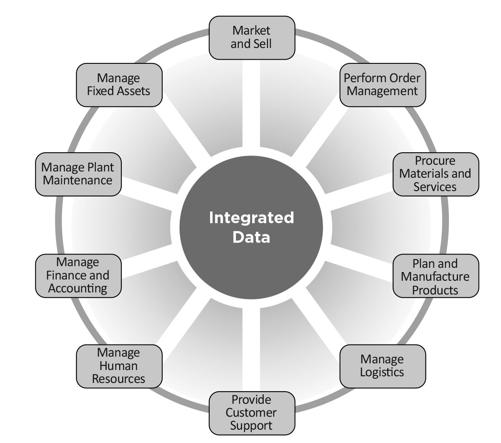
\includegraphics[scale=0.5]{Pictures/2_ERP_Processes.jpg}
    \caption{ERP-Supported Business Processes}
    \label{fig:2_ERP_Processes}
\end{figure}
\\
ERP systems are regarded as \textbf{cross-functional} in nature, since they satisfy the information needs of all end users, and also \textbf{process-centered} because they offer a clear, full, logical, and precise view of the business processes of the firm, which are groups of interconnected tasks that bring value to the enterprise.
Business operations frequently cross departmental boundaries and, in many circumstances, cross organizational boundaries, sharing data and information with external business partners like clients and suppliers, making ERPs essential within a company.
Some key business processes incorporated in ERP systems are shown in Figure \ref{fig:2_ERP_Processes}.

\section{Reasons for Implementing ERP}
Businesses that use ERP systems the most often have a lot of the same issues and frustrations. Figure \ref{fig:2_ERP_Reasons} lists the primary justifications for ERP adoption by businesses. A few of these reasons are explored below.

\begin{figure}
    \centering
    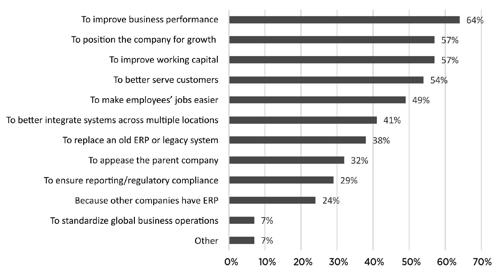
\includegraphics[scale=0.75]{Pictures/2_ERP_Reasons.jpg}
    \caption{Reasons for Implementing ERP}
    \label{fig:2_ERP_Reasons}
\end{figure}

\subsubsection{Improve business performance}
ERP improves business performance through the numerous best practices embedded within the several business processes. A \textbf{best practice} is a business procedure that is generally regarded as being more successful and/or efficient than others in a certain sector.
Companies that implement ERP will end up redesigning their previously disjointed, erroneous, slow, and ineffective processes to align with best practices in the software and can decrease operational costs, such as lower inventory costs, production costs, or purchasing costs, and increase revenue-generating processes, such as time to market, marketing and sales, and customer service.\\
Each view of best practices distinguishes one ERP vendor’s software from another’s, thus finding which ERP system's best practices match a buyer's demands is essential when choosing an ERP vendor's product since this fit influences the implementation's final success.
In order to find best practices across different industries and implement them into their solutions, the suppliers fund significant research and development (R\&D) initiatives. Additionally, it enables an ERP provider to provide niche versions of its software known as \textbf{vertical solutions}, which are essential due to the unique characteristics that each industrial sector has.

\subsubsection{Desire for growth}
Examples of growth strategies include market expansion and penetration, product diversification, and mergers and acquisitions (M\&A).
ERP systems help with market expansion through demand forecasting, which generates predictions to estimate the future requirements for items.
Advanced rule-based pricing is another feature of ERP software. This capability enables businesses to comprehend the present patterns and trends of the sector, consumers, and rivals before making any pricing modifications.
Businesses may expand their product lines and provide new items and features to their clients by diversifying their product offerings. Data on which items are selling and to whom may be found in ERP systems, as well as information on which products are just taking up space on the shelves.
Finally, an ERP may assist in standardizing procedures across organizations during an M\&A activity in order to integrate them into a common platform.

\subsubsection{Facilitate employees' work}
ERP systems are also recognized to make the duties of employees easier. ERP does this in part by providing employees with real-time access to information; this feature significantly enhances operations, corporate governance, and enterprise risk management, resulting in a horizontally "connected up," process-centered organization. ERP systems also offer an unified user interface and tool set that improves accuracy, encourages collaboration, and reduces misunderstanding. Finally, ERP systems empower users by providing them with access to data that was previously impossible to get due to fragmented procedures supported by many older systems.

\subsubsection{Lack of compliance}
Government and institutional compliance requirements continue to grow and evolve. Navigating through numerous legal, regulatory, and supply chain mandates has never been tougher. ERP systems can help companies comply with these requirements, such as GDPR, SOX or Food and Drug Administration.

\subsubsection{Data integration}
With ERP systems, data is better integrated since it is only gathered once and then shared throughout the company, reducing the risk of inaccuracies and duplications and eliminating time-consuming data checking, and reconciliation across systems. Because all users have access to up-to-date, accurate, and comprehensive data, this feature is advantageous to all of them. With ERP, since data is now kept in a single data repository, the process of fixing errors is made simpler because they only need to be fixed once.
Processes are also better integrated because they are managed within one system, not spread across multiple systems that have been cobbled together. When a corporation's systems are patched together from several sources, the scenario can cause problems on the operations designed to keep the organization functioning efficiently.

\subsubsection{Replacement an old ERP}
Having multiple disparate systems or operating an out-of-date ERP system, that runs on obsolete technology or that cannot support a company’s business processes, creates an IT maintenance nightmare. These systems may be complicated to customize, and installing fixes and upgrades can take up valuable time and resources. Additionally, because the vendor could no longer be in operation, it might not be viable to upgrade these systems.

\section{Disadvantages of ERP Systems}
An ERP system implementation is significantly more involved than merely installing commercially available software; it is a labor-intensive process that requires a variety of different tasks and, if managed incorrectly, might lead to the project's failure.
Companies shouldn't take the choice to deploy an ERP system lightly due of its importance. All workers, from functional users to IT professionals to top management, must be aware of the goals of the ERP project and collaborate to make the deployment successful.
Companies that are thinking about implementing an ERP system should perform due diligence in selecting the solution that best fits their needs and collaborating with experts who can help with different implementation-related tasks.

\subsubsection{People issues}
Top management can be a major problem if they do not establish a convincing “tone at the top” that the ERP system is a priority or if they don’t allocate adequate resources to its deployment.
Lack of support from the employees may also be a concern. The legacy systems that employees have used for years may make them feel quite at ease. They could oppose to the additional training, organizational adjustments, and modifications to business processes that are unavoidable, or they can claim that the system is too challenging, constrictive, or inflexible.
Employees who are resistant to the ERP system may create unproductive workarounds or create their own "shadow IT," such as spreadsheets or old systems, as a result of which they fail to use the system as intended.

\subsubsection{Software issues}
Because ERP systems are sophisticated and intricate, installing them sometimes necessitates paying high-priced system integrators. Companies frequently struggle to take control of technology and to use it to transform business processes in a quantifiable and sustainable way. A level of complexity that has not before been encountered and is difficult to absorb may also be added by the various capabilities, options, and setup requirements for businesses with relatively straightforward business requirements.

\subsubsection{Price tag}
ERP system deployments can cost millions of dollars and take years to complete, especially for big, international businesses. Additionally, once established, the ERP system requires ongoing "care and feeding" to keep it current, stable, and compatible with a variety of constantly evolving software programs with which it may interact. Companies often update and do larger improvements to the ERP system. This component of ERP might wind up costing more overall than the initial software licensing and implementation fees combined since maintenance charges are required annually.

\subsubsection{Standardization}
The above noted benefit of business process standardization may also be a drawback if the rigidity is inconsistent with the firm's culture or expectations. Additionally, a problem that must be resolved for the ERP installation to be effective is that the current corporate culture may not promote information exchange among business units or divisions. Vendors and system integrators actively advise businesses to adopt the best practices for ERP systems rather than customizing the software to fit their unique workflows. An exception, though, would be if businesses customized the software in accordance with a special business strategy that set them apart from rivals. The general guideline is that customizing the ERP software to get this capability is necessary if a certain procedure makes a business competitive or is required for compliance with a legislation.

\section{Modules}
ERP systems are offered as modules, which are collections of connected software applications that handle key organizational tasks like accounting or production. Each module is designed to support a particular business process.
The main modules, that provide basic functionalities for managing business processes, make up the \textbf{Core of the ERP}. This includes financial management, supply chain, human resources, customer relationship management, and other critical business processes. The "core" is the central and fundamental part of the ERP system and provides an integrated solution for managing company data.
Here are some of the most common modules found in ERP systems:
\begin{itemize}
    \item \textbf{Financial Management}: This module is responsible for managing financial transactions, such as accounts payable and receivable, general ledger, and financial reporting.
    \item \textbf{Accounting}: This module includes sub-modules for cost accounting, payroll, fixed asset management, and other accounting functions.
    \item \textbf{Human Resources}: This module manages employee information, benefits, payroll, and other HR functions.
    \item \textbf{Procurement}: This module covers all aspects of procurement, including vendor management, purchase order creation and management, and inventory management.
    \item \textbf{Supply Chain Management}: This module manages the flow of goods and services, including procurement, production, and logistics.
    \item \textbf{Production}: This module helps manage the production process, including planning, scheduling, and tracking.
    \item \textbf{Sales and Marketing}: This module supports sales and marketing activities, including lead management, opportunity tracking, and customer relationship management.
    \item \textbf{Customer Relationship Management (CRM)}: This module supports customer-facing activities, such as marketing, sales, and customer service.
\end{itemize}
The specific modules included in a particular ERP system can vary based on the size of the
organization and its unique business requirements. Most ERP software is flexible enough to allow
businesses to purchase only the components they require “a la carte”, this allows companies to have
a solution “tailor-made” to its needs. Modular architecture has the advantage of enabling ERP
suppliers to create product solutions for specific industries. Sometimes modules that support a
major business area are called a \textbf{suite} which comprises multiple sub-modules, or components.
An example is shown in Figure \ref{fig:3_ERP_Modules}, where ERP modules for a manufacturing company
are depicted.
\begin{figure}
    \centering
    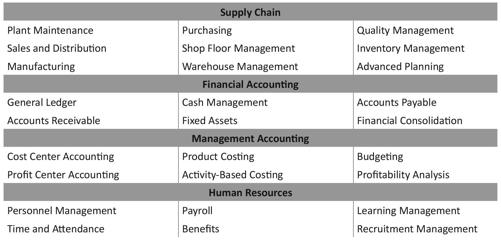
\includegraphics[scale=0.75]{Pictures/3_ERP_Modules.jpg}
    \caption{Examples of ERP Modules for a manufacturing company}
    \label{fig:3_ERP_Modules}
\end{figure}
\\
In summary, the various modules in an ERP system work together to provide a comprehensive solution
for managing business processes and data. By integrating all business functions into a single
system, organizations can streamline processes, reduce data duplication, improve business analytics,
and make more informed decisions.

\section{Technology}
An ERP system has a far-reaching impact that affects users across an entire organization, as well as
its customers, suppliers, and other business partners. With the need to support a large number of
users who have different processing and reporting requirements, it is important to have advanced and
adaptable software that utilizes cutting-edge technology. Given that the ERP system plays a crucial
role in fulfilling an organization's operational and information needs, it is essential to have a
thorough understanding of the technology that supports the integrated system, and provide a robust,
scalable, and user-friendly solution for managing a wide range of business processes and data.

\subsection{Three-Tier Client-Server Architecture}
The client-server architecture\textsuperscript{\cite{web_application}} is widely used in modern
computing, and is a fundamental aspect of many systems, including ERP systems. This architecture is
a computing model in which a server (\textbf{Back-end application}) provides services to clients
(\textbf{Front-end application}) over a network. The client requests a service or resource from the
server, and the server responds by providing the requested information or performing the requested
task. This architecture allows for efficient and scalable distribution of resources and tasks, as
the server can handle requests from multiple clients simultaneously.
\newline\newline
In this context we can separate an application into three logical components \textbf{(3-Tier
    architecture)}, which are the client tier, the application tier, and the database tier. This
architecture provides a scalable, flexible, and secure solution for software applications. In Figure
\ref{fig:2_ERP_arch} is showed a detailed explanation of each tier.

\begin{figure}\centering
    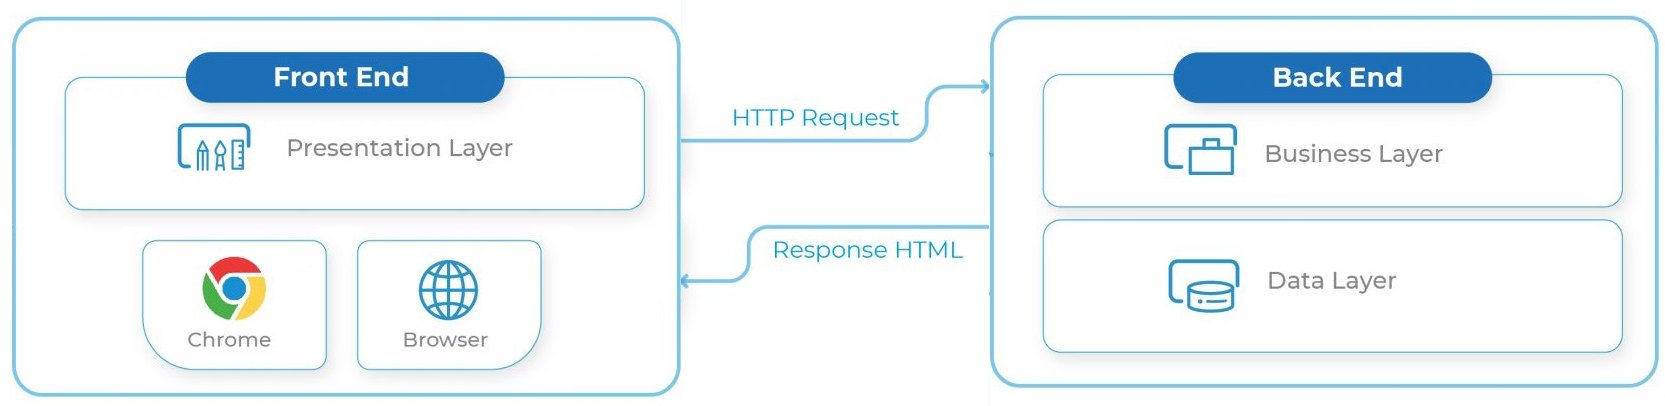
\includegraphics[scale=0.33]{Pictures/2_ERP_arch.jpg}
    \caption{Web Application Architecture}
    \label{fig:2_ERP_arch}
\end{figure}

\begin{itemize}
    \item \textbf{Client Tier - Presentation layer}: This tier is responsible for presenting the user interface to the end-user. It provides the interface through which users interact with the application. The client tier can be implemented as a standalone application or as a web application accessed through a web browser.
    \item \textbf{Application Tier - Business layer}: This tier is responsible for processing the user requests and returning the results to the client tier. It is responsible for handling the business logic and data processing. The application server tier is typically implemented as a web server.
    \item \textbf{Database Tier - Data access layer}: This tier is responsible for storing and managing the vast amount of data generated by the application. It is a key component of a web application that stores and manages information for a web app. You can search, filter and sort information based on user request. It is typically implemented using a robust database management system.
\end{itemize}
The three-tier architecture allows for a separation of concerns, with each tier having a specific role and responsibility. This separation makes it easier to develop, maintain, and upgrade the application, as changes can be made to one tier without affecting the others. Additionally, by dividing the system into separate tiers, the performance and security are improved. The client does not have direct access to the data, instead, all data passes through the application server which controls and regulates access to the information. This allows for more efficient and secure management of data. The ability to deploy application servers on multiple machines provides higher scalability, better performance and better re-use. \\
The Three-Tier Client-Server Architecture is a widely used architecture for ERP systems, as it provides a scalable, flexible, and secure platform for managing complex business processes and data.


\subsection{Deployment}
An ERP system can be deployed in two ways: On-premise or on Cloud, each with its own advantages and disadvantages. The best deployment method depends on the specific needs and requirements of the organization.

\subsubsection{On-Premise}
The conventional approach to ERP deployment is \textbf{on-premise ERP}.
In this deployment method, the ERP software is installed and run on computers within an organization's own physical facilities. This allows for complete control over the software and data, but also requires the organization to provide the necessary hardware, storage, and technical support. Companies choosing the “on-prem” option are usually larger companies with bigger budgets, an existing IT infrastructure in place, and knowledgeable IT personnel to support the software and infrastructure. Due to the large upfront cost required, which often includes the cost of both hardware and software, on-premise ERP is typically seen as a capital investment.

\subsubsection{Cloud}
\textbf{Cloud ERP} deployment is becoming increasingly popular, where the ERP system is hosted by a vendor or third party on shared computing resources that can be accessed through the internet. These resources are maintained in data centers dedicated to hosting various applications on multiple platforms.
This deployment method offers more scalability and flexibility, as well as reduced hardware and technical support expenses, but it requires an organization to have trust in a third party with access to its data.
Customers have access to the ERP system as needed and pay for the software on a monthly or yearly basis. This method of paying for ERP software on a subscription basis is called \textbf{software as a service (SaaS)}, an attractive option for businesses looking to reduce upfront expenses and to budget for ERP long-term.
Nowadays, nearly all ERP vendors offer some form of cloud deployment because it has many advantages compared to on-premise deployment.

\subsubsection{Advantage}
\begin{itemize}
    \item One key advantage is that ERP cloud providers maintain, upgrades and handle maintenance for the infrastructure of the ERP system.
    \item Cloud ERP is more scalable than on-premise, which is ideal for startups and fast-growing businesses.
    \item Companies that choose cloud ERP over on-premise can now enjoy more peace of mind that the cloud provider has up-to-date controls in place such as data backup, dual factor authentication, encryption for confidential data, and a disaster recovery plan.
\end{itemize}

\subsubsection{Disadvantages}
\begin{itemize}
    \item Many vendors offering cloud solutions are primarily focused on just one particular area. Very few cloud providers are offering a suite of products to meet the needs of medium-to-large organizations.
    \item Many cloud ERP solutions are limited in what the customer can do in terms of customization.
    \item Although cloud ERP is generally thought to be less expensive than on-premise, research has shown that over a 10-year window, the total costs for each converge. While expenses for cloud ERP are less upfront than on-premise, the costs catch up over time. Thus, the costeffectiveness of cloud ERP is not as great as initially thought.
\end{itemize}

\subsection{Customization}
It's uncommon for an ERP system to fully meet a company's needs, especially if the company is a large, global organization. There are often problems that go beyond what the ERP software can accommodate through configuration. Examples of these issues include:
\begin{itemize}
    \item Creating additional functionality not provided by the ERP system \item Establishing connections between the ERP system and third-party systems
    \item Adding extra fields to the ERP database
\end{itemize}
These types of problems usually require development and programming to enhance the ERP system. This is known as customization, which involves adding custom code to increase the capabilities and features of the ERP system. Customization is typically performed when all efforts to find a solution through configuration have failed. As customization requires time and money, companies should aim to minimize it.

\section{Market}
The ERP market is estimated at \$43.72 billion in 2020, and is projected to reach \$117.09 billion
by 2030, at a compounded annual growth rate of 10.0\%\textsuperscript{\cite{erp_market}}. The increase in the ERP market can be
attributed to the growing interest from small and medium-sized businesses and the development of new
ERP applications for both cloud and mobile platforms. However, not all ERP vendors offer the same
quality of software, which can be divided into three categories based on specific criteria, as
presented in a table \ref{tab:table_ERP_Tiers}.
\begin{itemize}
    \item \textbf{Tier I} (Enterprise Class) is software designed for large, worldwide corporations with significant market capitalization and annual revenues that exceed \$750 million. These solutions are very costly due to their extensive capabilities, including the ability to manage complex organizational structures and address international concerns, like multiple currencies and varying accounting regulations. Only a few ERP vendors have the necessary size, resources, and comprehensive functionality to support the high volume of daily transactions that Tier I companies typically encounter.
    \item \textbf{Tier II} (the Mid-Market Class) category of ERP systems is intended for medium-sized companies and can be further divided into upper and lower sub-categories. Upper Tier II systems are for companies with annual revenues ranging from \$250 million to \$750 million. Lower Tier II systems typically are for companies with annual revenues between \$10 million and \$250 million.
          These vendors offer software that is designed for either single or multiple legal entities and locations, but with limited functionalities compared to Tier I vendor solutions. As a result, these ERP systems are less expensive than Tier I systems. Typically, they are easier to implement and support and are designed specifically for only a few industries.
    \item \textbf{Tier III} (Small Business Class) ERP systems are made for smaller businesses with annual revenue below \$10 million, operating within a single country. They are the most affordable among the different tiers of ERP systems. The market is saturated with many software providers in this category, some of which offer robust point solutions that can be utilized to enhance a Tier I or Tier II ERP system.
\end{itemize}
\begin{table}
    \centering
    \begin{tabular}{p{4.4cm} | p{4.4cm} | p{4.4cm}}
        \hline\hline
        Tier I                       & Tier II                          & Tier III                              \\
        \hline
        %\hspace*{1.3em}
        High complexity              & Medium complexity                & Low complexity                        \\
        Highest cost                 & Medium cost                      & Lowest cost                           \\
        Many industry solutions      & Fewer industry solutions         & Fewest industry solutions             \\
        Large companies              & Mid-market companies             & Small companies                       \\
        Support global functionality & Operate in more than one country & Does not support global functionality \\
        \hline \hline
    \end{tabular}
    \caption{Characteristics of ERP Vendor Tiers}
    \label{tab:table_ERP_Tiers}
\end{table}
The ERP market is experiencing a trend where Tier II and Tier III vendors are aiming to serve larger companies by improving their software's capabilities and scalability, while Tier I vendors are reaching smaller companies by offering simplified versions of their software and acquiring cloud vendors. This is causing the boundaries between ERP tiers to become less distinct as vendors strive to increase their market share.
Table \ref{tab:table_ERP_vendor} presents some example of ERP systems in  tiers.
\begin{table}
    \centering
    \begin{tabular}{p{4.4cm} | p{4.4cm} | p{4.4cm}}
        \hline\hline
        Tier I      & Tier II                 & Tier III \\
        \hline
        SAP S4/HANA & Microsoft Dynamics 365  & Sage     \\
        Oracle EBS  & NetSuite                & Aptean   \\
        Infor LN    & SAP Business All-in-One & ASC      \\
        Infor M3    & ODOO                    & ECI      \\
        \hline \hline
    \end{tabular}
    \caption{Example ERP Vendors in Tiers}
    \label{tab:table_ERP_vendor}
\end{table}

\subsection{Cost}
%articolo "Be Wary of the Economics of Serverless Cloud Computing"
%documento pricing guide BC
Numerous ERP projects run over budget, often as a result of unanticipated organizational or
technological problems, scope expansion, or an unrealistic project budget. Budgeting for ERP can be
difficult since some costs are difficult to predict at first. This section will go into depth about
every expense that goes into calculating the system's total cost of ownership \textbf{total cost of
    ownership (TCO)}. Some of these costs will be one-time costs, while others will be
recurring\textsuperscript{\cite{erp}}.

\subsubsection{Software License Costs}
Typically, an ERP system’s price tag depends on the:
\begin{itemize}
    \item Number of employees that will be using the system
    \item Vendor tier being deployed, Tier 1 software is more expensive than Tier 2, while Tier 3 would be the least expensive
    \item Number of modules purchased
\end{itemize}
The vast majority of ERP software licenses are supplied using a \textbf{perpetual licensing model}, which requires paying an upfront licensing price before the vendor grants access to the program for an endless amount of time. Additionally, customers must pay annual maintenance costs in order to get support, updates, and future software upgrades. For on-premise implementations, perpetual licensing is standard. With perpetual licensing, a couple of license methods are used:
\begin{itemize}
    \item \textbf{Named user licensing}. A company determines how many unique users will use the ERP system and pays a licensing charge for each of them. Numerous ERP vendors provide different named user categories, such as heavy user licensing, for users who utilize more system capability and are thus paid a larger license fee, or casual user licensing, for users who just read reports or lists.
    \item \textbf{Concurrent user licensing}. A perpetual license type enables an unlimited number of designated users and accounts, but restricts the number of individuals who can actively use the software at one time. Concurrent user licensing is often cheaper than named user licensing as it only requires payment for the estimated number of simultaneous users. However, it's essential to accurately predict the number of concurrent users, otherwise, employees may experience difficulties logging on and using the software.
\end{itemize}

\subsubsection{Third-Party Software License Costs}
In some cases, a company has specific requirements that cannot be fulfilled by the ERP system they have purchased, and modifying the ERP to meet those requirements is too costly. To address this, third-party software known as "bolt-ons" can be used. These provide additional functionality or logic to help solve specific business needs. To ensure seamless integration with the ERP system, it is advisable to get recommendations from the ERP vendor or system integrator on which bolt-on solution will work best.

\subsubsection{Hardware and IT Infrastructure Costs}
The implementation of an ERP system requires a strong and up-to-date IT setup. If the ERP is run on-site, a company will need to invest in IT hardware such as servers, routers, backup, storage devices, desktops, laptops, tablets, and printers. They will also need to consider measures for failover, network access, power supply, and security. This may involve hiring additional staff and increasing data center space, with costs ranging from one-time expenses like purchasing servers to ongoing expenses like utility bills and salaries.

\subsubsection{Database License Costs}
The cost of the database in an ERP project can range from a few thousand dollars to hundreds of thousands of dollars, depending on several factors such as the type of database, the size of the data being stored, and the number of users accessing the database. ERP vendors will provide the specifications for the type of database needed.

\subsubsection{Implementation Costs}
The expenses related to the implementation of ERP software are among the most pricey parts of the total cost of ownership (TCO). The cost of functional and technical consultants, who play a key role in the implementation, can be a major part of these expenses, depending on how much a company is going to rely on the system integrator.
The complexity of the project and consultants from different geographical locations may also affect the hourly rate charged.

\subsubsection{Maintenance and Support Costs}
The cost of an ERP system doesn't end once the software is up and running. To ensure the system continues to run smoothly, companies need to have a plan for ongoing maintenance and support, also known as \textbf{application management services (AMS)}. This includes functional and technical support, updating and patching, monitoring the software, and backup and recovery. Some companies can handle these tasks in-house, while others may hire a third-party company to provide these services. The cost of maintenance typically ranges from 18\% to 25\% of the original software license cost and can be paid directly to the ERP vendor or to the third-party company managing the system. \\
For software support, various levels are available, with the higher levels offering more services at a higher cost. Premium support could include having a representative from the ERP vendor on-site during the project implementation and for a period of time post-implementation, as well as prioritized access to help tickets. Basic support might only provide access to a help portal where customers can log tickets and get answers to questions.

\subsubsection{Cloud}
The Total Cost of Ownership (TCO) in a cloud context is the same as what we previously discussed,
but often, all of the costs are included in a single \textbf{subscription-based licensing}.
Customers subscribing to this model are granted program access for a set duration, such as monthly
or annually, which covers not only the use of the software but also maintenance, support, scheduled
updates, and upgrades provided by the cloud vendor. This comprehensive subscription often includes a
basic database offering, with the flexibility to expand storage for an additional fee.
\newline\newline
Predominantly, ERP applications are marketed as \textbf{Software as a Service (SaaS)}, a cloud-based
delivery model wherein the vendor shoulders the responsibility for the underlying infrastructure,
including hosting, maintenance, and support. This implies that the costs for IT infrastructure, when
the ERP system is hosted by the vendor or a third-party provider, are bundled into the monthly
subscription fee. Companies utilizing public cloud platforms like Microsoft Azure would typically
pay a recurring fee for the infrastructure lease in addition to the software licensing fees due to
the ERP vendor.

\subsection{Competitors}
The ERP (Enterprise Resource Planning) market is experiencing a significant shift with the emergence
of smaller, more agile players. These smaller vendors are challenging the traditional dominance of
larger, established companies like SAP, Oracle, and Microsoft. Characterized by their innovative,
cloud-native solutions, these emerging players focus on delivering specialized and industry-specific
ERP systems. This approach contrasts with the one-size-fits-all, monolithic systems traditionally
offered by the larger vendors\textsuperscript{\cite{erp_competitor_1}}.
\newline\newline
This trend towards smaller, more nimble ERP vendors is driven by the increasing popularity of
cloud-based solutions. These solutions offer benefits such as lower costs, greater scalability, and
flexibility, making them particularly appealing to small and medium-sized enterprises. The pandemic
has further accelerated this shift, as businesses seek solutions that support remote work and offer
greater operational agility. As a result, the ERP market is becoming more fragmented and
competitive, providing businesses with a wider array of choices to suit their specific
needs\textsuperscript{\cite{erp_competitor_2}}.
\newline\newline
This section provides an overview of the key features of some cloud ERP products based on research
from the ERP Research comparison platform\textsuperscript{\cite{erp_research}}. These features are
critical for businesses to consider when choosing an ERP system, as they directly impact usability,
scalability, and overall business efficiency.

\subsubsection{SAP Business One}
\begin{table}
    \centering
    \begin{tabular}{|p{0.45\textwidth}|p{0.45\textwidth}|}
        \hline
        \textbf{PROS} & \textbf{CONS}                                             \\ \hline
        \begin{itemize}
            \item A complete business management solution for SMEs.
            \item Exceptional performance in handling business functions.
            \item Simple user interface and internal controls.
            \item Can be highly customized to adapt to business needs.
            \item Mature product with major functionalities supported.
            \item Deployment flexibility for On-Prem, SaaS or Private Cloud.
        \end{itemize}
                      &
        \begin{itemize}
            \item Limited Human Capital and Manufacturing functionalities supported.
            \item The limitation to customize the dashboards and cockpit feature.
            \item The Firefox web browser is currently the only web browser supported.
            \item Heavy reliance on partner addons for deeper and wider functionality.
            \item Requires heavy customization which can lead to IT debt.
        \end{itemize} \\ \hline
    \end{tabular}
    \caption{Pros and Cons of SAP Business One.}
    \label{tab:sap_pros_cons}
\end{table}

\newpage

\subsubsection{Microsoft Dynamics 365}
\begin{table}
    \centering
    \begin{tabular}{|p{0.45\textwidth}|p{0.45\textwidth}|}
        \hline
        \textbf{PROS} & \textbf{CONS}                                  \\ \hline
        \begin{itemize}
            \item Good integration with other software and technologies.
            \item User friendly, easy to train users.
            \item Secure and permission-based account setup.
            \item Flexible and customizable for all company needs.
            \item Extensive filtering capabilities.
        \end{itemize}
                      &
        \begin{itemize}
            \item Difficult migration from old ERP.
            \item Some functions could be more user friendly and intuitive.
            \item User documentation needs improvement.
            \item Can be expensive due to high level of customization.
        \end{itemize} \\ \hline
    \end{tabular}
    \caption{Pros and Cons of Microsoft Dynamics 365.}
    \label{tab:microsoft_pros_cons}
\end{table}

\subsubsection{ODOO}
\begin{table}
    \centering
    \begin{tabular}{|p{0.45\textwidth}|p{0.45\textwidth}|}
        \hline
        \textbf{PROS} & \textbf{CONS}                                                               \\ \hline
        \begin{itemize}
            \item Low-cost when investing in a small number of modules.
            \item Free "Community" version available.
            \item Offers a comprehensive selection of Odoo apps and integrates with many thirdparty add-on software apps.
            \item Uses Open Source software which can be easily customized.
        \end{itemize}
                      &
        \begin{itemize}
            \item Requires IT knowledge to install and maintain, this is not a "plug and play" solution.
            \item Steep learning curve on initial implementation.
            \item Costs may rise with the use of numerous Odoo Modules and third-party apps.
            \item Has a shorter history compared to other established ERP players.
        \end{itemize} \\ \hline
    \end{tabular}
    \caption{Pros and Cons of ODOO platform.}
    \label{tab:odoo_pros_cons}
\end{table}

\newpage

\subsubsection{Oracle NetSuite}
\begin{table}
    \centering
    \begin{tabular}{|p{0.45\textwidth}|p{0.45\textwidth}|}
        \hline
        \textbf{PROS} & \textbf{CONS}                                                                                         \\ \hline
        \begin{itemize}
            \item Wide and deep functionality across several key business areas.
            \item True SaaS Cloud ERP offering.
            \item Largest Cloud ERP customer base and ecosystem.
            \item Strong localization capabilities for international businesses.
            \item Strong consultant market and availability.
        \end{itemize}
                      &
        \begin{itemize}
            \item License pricing is complex and can produce hidden costs.
            \item Some localisations and functionality is not provided out of the box put as part of partner extensions.
            \item Many acquisitions have led to the solution being more loosely connected instead of a cohesive, integrated suite.
            \item Strong consultant market and availability.
        \end{itemize} \\ \hline
    \end{tabular}
    \caption{Pros and Cons of Oracle NetSuite.}
    \label{tab:oracle_pros_cons}
\end{table}

\chapter{Fundamentals}
In this chapter, we embark on a journey to construct the narrative foundation that underpins our
thesis. Here, we will introduce the essential design concepts and the innovative technologies that
have been employed in the creation of the platform known as Kube. This platform is envisioned as an
ERP system that not only encapsulates the core functionalities typical of such software but also
adopts a serverless and microservice architecture. To achieve this, we will delve into the process
of fragmenting the ERP into smaller, more manageable modules. These modules will then be intricately
woven together and seamlessly integrated within a FaaS (Function as a Service) model environment,
exemplified by services such as AWS Lambda. This integration is key to realizing a system that is
both highly modular and scalable, leveraging the agility afforded by serverless computing and the
robustness of microservices. Through this exploration, we aim to provide a detailed understanding of
both the design philosophy and the technological framework that define the functionality and
innovation of Kube.

\section{Cloud Computing}
The advent of cloud computing has revolutionized the way we approach computing and data management.
This section of the thesis will explore the paradigm of cloud computing, which has emerged as a
transformative force in the technological landscape. We will examine the fundamental aspects of
cloud computing, including its service models, deployment strategies, and the pivotal role it plays
in modern IT infrastructure.

\subsection{Definition}
The United States National Institute of Standards and Technology's definition of cloud computing
is\textsuperscript{\cite{nist}}:

\begin{quote}
    Cloud computing is a model for enabling ubiquitous, convenient, on-demand network access to a
    shared pool of configurable computing resources (e.g., networks, servers, storage, applications, and
    services) that can be rapidly provisioned and released with minimal management effort or service
    provider interaction. This cloud model is composed of five essential characteristics, three service
    models, and four deployment models.
\end{quote}

Cloud computing offers a highly flexible service delivery model, enabling on-demand access to
various resources, such as storage, processing power, and applications, via the internet. This
eliminates the need for local servers, shifting data handling to online remote servers and offering
a cost-effective, pay-for-what-you-use pricing model. Services like Amazon Web Services (AWS)
provide the technology infrastructure, allowing users to scale operations with ease. Additionally,
this model promotes economic efficiency, as organizations pay only for resources they consume,
supporting a scalable and agile approach to resource management. The network, often the internet,
serves as a conduit between users and cloud services, ensuring data is managed with strong security
measures.

\subsubsection{Essential Characteristics}
Five essential characteristics of cloud computing are\textsuperscript{\cite{nist}}:
\begin{itemize}
    \item \textbf{On-Demand Self-Service}: Users can independently set up and manage their computing needs, such as
          server time and network storage, automatically, eliminating the need for direct interaction with
          service providers.
    \item \textbf{Broad Network Access}: Services are accessible over the internet using standard methods that
          support a diverse range of devices, including smartphones, tablets, laptops, and desktops.
    \item \textbf{Resource Pooling}: The provider's computing resources are aggregated to serve various customers
          under a multi-tenant model. Resources are dynamically allocated and reallocated based on user
          demand, with the user typically not knowing or controlling the exact physical location of the
          resources but may be able to designate a location at a broader level (such as country, state, or
          data center).
    \item \textbf{Rapid Elasticity}: Services can be quickly scaled up or down to match demand, with the scaling
          process sometimes occurring automatically. From the user's perspective, the supply of available
          resources often seems boundless and can be acquired in any volume at any time.
    \item \textbf{Measured Service}: Cloud platforms automatically monitor, control, and report resource usage with
          a metering function that operates at an appropriate level of detail, depending on the type of
          service, such as storage space, processing power, bandwidth, or active user numbers. This metering
          provides clear visibility into the usage of services for both the provider and the consumer.
\end{itemize}

\subsection{Service Models}
Cloud computing has revolutionized the way businesses approach technology, offering a spectrum of
services that cater to varying requirements for control, flexibility, and management. As
organizations transition to cloud-based solutions, understanding the different service models
becomes crucial for leveraging the full potential of the cloud.

The figure \ref{fig:3_cloud_models} shows the three primary cloud service models, forming what is
often referred to as the cloud computing "stack," include Infrastructure as a Service (IaaS),
Platform as a Service (PaaS), and Software as a Service (SaaS). These service models are designed to
build upon one another, offering layers of abstraction and increasing levels of managed
services\textsuperscript{\cite{cloud_amazon}}.

\begin{figure}
    \centering
    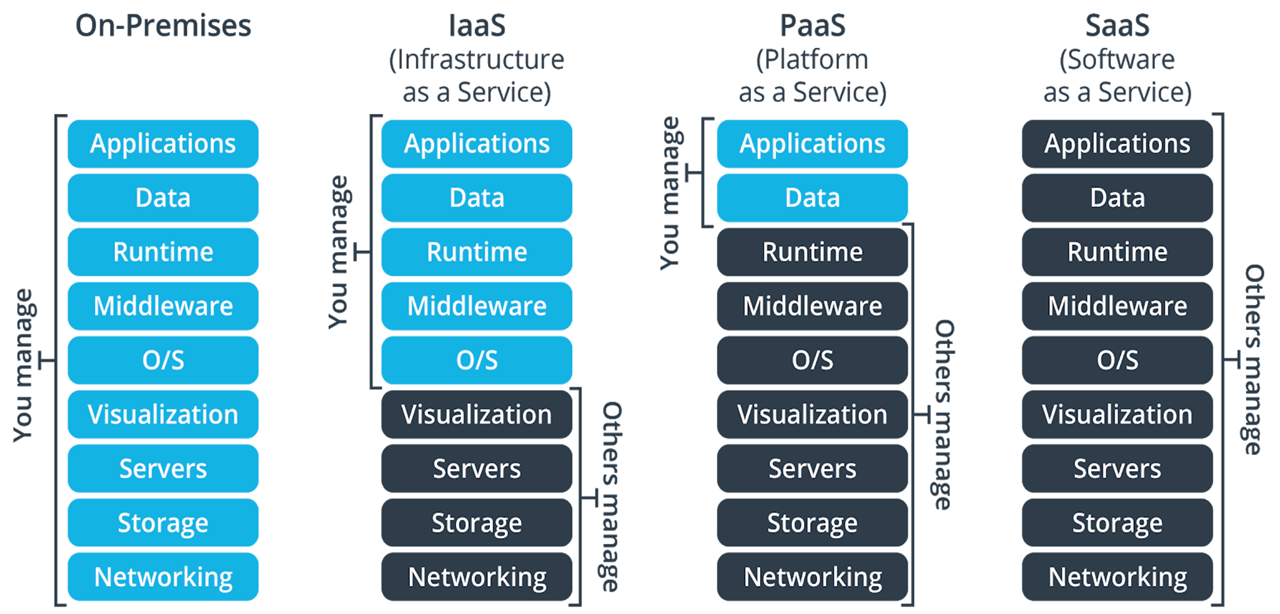
\includegraphics[scale=0.25]{Pictures/3_cloud_models.png}
    \caption{Cloud service models \textsuperscript{\cite{cloud_models}}.}
    \label{fig:3_cloud_models}
\end{figure}

\subsubsection{Infrastructure as a Service (IaaS)}
Infrastructure as a Service (IaaS) is a transformative approach to managing IT resources, offering
flexible and on-demand access to essential infrastructure services through the internet. This
includes virtual machines, storage, and networking that can be customized and billed based on actual
usage. IaaS grants organizations unprecedented control over their IT resources, closely resembling
traditional on-premises infrastructure. It allows for easy scalability without the need for costly
upfront investments in hardware. IaaS empowers consumers with the ability to provision processing,
storage, and networking resources, deploying and running various software, including operating
systems and applications. This level of customization enables organizations to tailor their IT
environment to their specific needs, ensuring a seamless and efficient operation in the cloud.

\subsubsection{Platform as a Service (PaaS)}
Platform as a Service (PaaS) is a significant innovation in cloud computing, offering comprehensive
hardware and software resources for cloud-based application development. Leading PaaS providers
simplify development by effectively managing the underlying infrastructure, allowing a laser focus
on application creation. With PaaS, you're free from infrastructure oversight, enabling dedicated
attention to application deployment and management, improving operational efficiency by eliminating
resource provisioning, capacity planning, and maintenance. PaaS provides an environment for
building, testing, and managing software applications without the need to manage the underlying
cloud infrastructure. As a user, you control your applications and their hosting settings,
simplifying the development process by allowing you to focus solely on creating and deploying your
applications.

\subsubsection{Software as a Service (SaaS)}
Software as a Service (SaaS) is a cloud computing model that delivers software applications over the
internet on a subscription basis. In this approach, cloud providers manage and host the
applications, ensuring their availability, performance, and security. Well-known examples of SaaS
offerings include Google Workspace, Microsoft Office 365, and Salesforce. SaaS provides a complete
software solution over the internet, including the application and its underlying infrastructure,
which is fully maintained by the cloud service provider. This approach spares users from managing
the infrastructure, as the provider handles software updates and security measures. Users can access
these applications through different devices and web browsers, enjoying an accessible and simplified
experience. SaaS enables users to efficiently utilize applications hosted on the cloud, focusing
solely on using the software rather than its maintenance.

\subsection{Deployment Models}
% possibile immagine da qui https://www.slideteam.net/cloud-computing-deployment-models-cloud-service-models-it.html
Cloud computing, a key driver in modern IT resource management, offers various deployment models
tailored to different business needs, security requirements, and scalability demands. This
exploration focuses on Public, Private, Hybrid, and Community Cloud models, discussing their unique
features, benefits, and considerations.

\subsubsection{Community Cloud}
Community-dedicated cloud infrastructure is exclusively used by a specific community of
organizations with shared interests, including mission objectives, security requirements, policies,
and compliance regulations. This infrastructure can be managed by one or more organizations within
the community, external providers, or a combination of both, and it can be located on-premises or
off-premises to accommodate community preferences\textsuperscript{\cite{nist}}.

\subsubsection{Private Cloud}
A private cloud is a form of cloud computing providing exclusive resources and services via a
private network, dedicated solely to one organization. It offers enhanced security and data
isolation, with the ability to tailor infrastructure and software to specific needs and workflows.
While offering robust security and control, private clouds can be costlier due to the organization's
responsibility for infrastructure management and scaling. These can be deployed on-site or hosted by
third-party providers, catering specifically to businesses requiring high security and compliance
standards. The combination of cloud computing benefits with heightened data security and
customization makes private clouds an attractive option for businesses handling sensitive data.

\subsubsection{Public Cloud}
In public cloud computing, a third-party service provider manages all the level of infrastructure,
including servers, storage, and computing resources. Clients access these resources via the internet
and are billed based on their actual usage, creating a cost-effective and flexible pay-as-you-go
model. These cloud environments eliminate the need for substantial investments in expensive
infrastructure, democratizing access to cloud computing. It's important to note that public clouds
operate on shared infrastructure, which offers cost efficiencies but raises concerns about data
isolation and privacy, as multiple customers' data and applications coexist on the same
infrastructure.

\begin{figure}
    \centering
    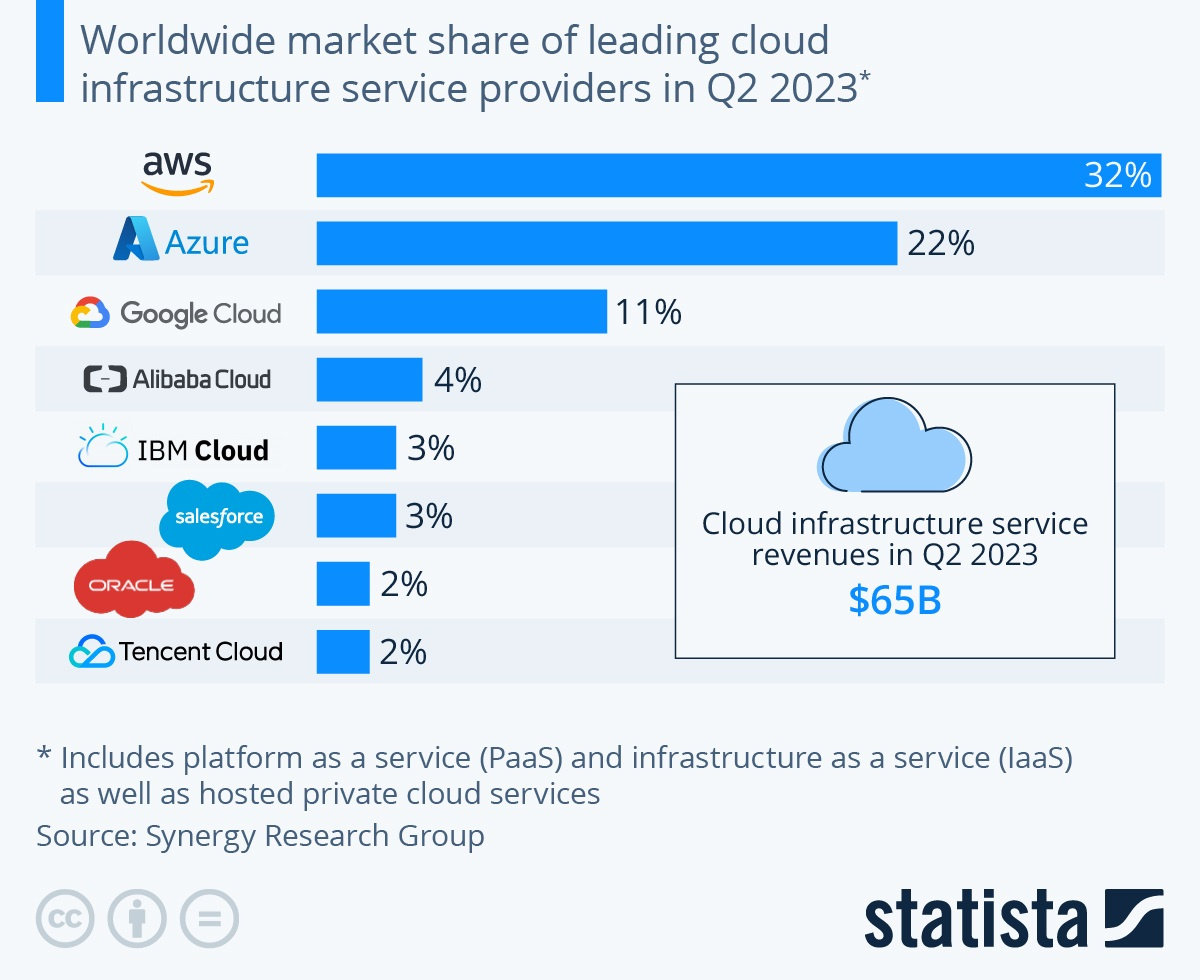
\includegraphics[scale=0.25]{Pictures/3_cloud_vendors.png}
    \caption{Worldwide market share of leading cloud infrastructure service providers in Q2 2023\textsuperscript{\cite{market_cloud_vendors}}.}
    \label{fig:3_cloud_vendors}
\end{figure}

The figure \ref{fig:3_cloud_vendors} show how the public cloud marketplace consists of numerous
cloud providers. Amazon, Microsoft and Google account for 65\% of the total 2023 cloud market. The
remaining public cloud market is divided among IBM, Alibaba, Oracle and several smaller players. The
table \ref{tab:cloud_providers} make a comparison between the major cloud providers.

\begin{table}
    \centering
    \begin{tabular}{|l|c|p{3.8cm}|p{3.8cm}|}
        \hline
        \textbf{Name}            & \textbf{Cost/hour} & \textbf{Pros}                              & \textbf{Cons}                                            \\ \hline
        \textbf{Amazon AWS}      & \$0.0255           & Reliability, Quality, Professional Support & Expensive despite regular lowering of price              \\ \hline
        \textbf{Google GCP}      & \$0.0475           & Reliability, Affordable                    & Limited features and services                            \\ \hline
        \textbf{Microsoft Azure} & \$0.043            & Best infrastructure configuration          & Unsatisfactory customer experience and technical support \\ \hline
        \textbf{IBM Cloud}       & \$0.04             & Flexibility, Speed, Interoperability       & Complicated pricing model and platform can be slow       \\ \hline
    \end{tabular}
    \caption{Comparative overview of major cloud service providers\textsuperscript{\cite{top_cloud_vendors}}.}
    \label{tab:cloud_providers}
\end{table}

\subsubsection{Hybrid Cloud}
The hybrid cloud is an advanced cloud computing model that blends public and private clouds, giving
organizations the flexibility to distribute their applications and workloads as needed. This setup
allows for greater control and scalability than using only public clouds, letting businesses keep
sensitive data secure while still enjoying public cloud efficiency. It's ideal for companies that
need both strong security and the ability to quickly adapt and scale. The hybrid cloud offers a
versatile IT infrastructure that adjusts to the complex needs of modern businesses, improving
security, compliance, and overall efficiency. This makes it a valuable asset for companies
navigating the rapidly changing digital world.

\subsection{Benefits}
Cloud computing is a big shift from the traditional way businesses think about IT resources. Here
are seven common reasons organizations are turning to cloud computing services\textsuperscript{\cite{cloud_azure}}:

\begin{itemize}
    \item \textbf{Cost}: Cloud computing reduces the capital expense of buying hardware and
          software, setting up and running on-site datacenters, which can quickly add up.
    \item \textbf{Speed}: Cloud services are typically on-demand, allowing vast amounts of computing
          resources to be provisioned in minutes, offering businesses flexibility and easing capacity
          planning.
    \item \textbf{Global Scale}: It includes the ability to elastically scale IT resources,
          providing the right amount of computing power, storage, and bandwidth when and where needed.
    \item \textbf{Productivity}: Cloud computing eliminates many time-consuming tasks associated
          with managing on-site datacenters, allowing IT teams to focus on more important business goals.
    \item \textbf{Performance}: Cloud services run on a worldwide network of secure datacenters,
          regularly upgraded to the latest generation of fast and efficient computing hardware, offering
          benefits like reduced network latency and greater economies of scale.
    \item \textbf{Reliability}: Data backup, disaster recovery, and business continuity are easier
          and less costly, as data can be mirrored at multiple redundant sites on the cloud provider’s
          network.
    \item \textbf{Security}: Cloud providers typically offer a broad set of policies, technologies,
          and controls to strengthen security, protecting data, apps, and infrastructure from threats.
\end{itemize}

\subsection{Market Overview}
The global cloud computing market, valued at USD 483.98 billion in 2022, is expected to exhibit a
robust compound annual growth rate (CAGR) of 14.1\% from 2023 to
2030\textsuperscript{\cite{market_cloud_computing}}. This remarkable growth is attributed to the
cloud's capacity to significantly enhance business performance in large enterprises, the increasing
demand for hybrid and Omni-cloud systems, and the adoption of pay-as-you-go models. Cloud services
have gained popularity in developing countries, thanks in part to government initiatives aimed at
safeguarding data integrity and security. The COVID-19 pandemic has expedited the adoption of cloud
computing, driven by the shift towards hybrid work models. While data privacy and security concerns
remain, large enterprises are increasingly turning to cloud-based technologies to optimize costs.
Moreover, cloud adoption is on the rise among small and medium-sized organizations, and governments
in developing nations are making substantial investments in cloud delivery models to enhance
productivity. The Figure \ref{fig:3_cloud_computing_market} illustrates the growth of the U.S. cloud
computing market.

\begin{figure}
    \centering
    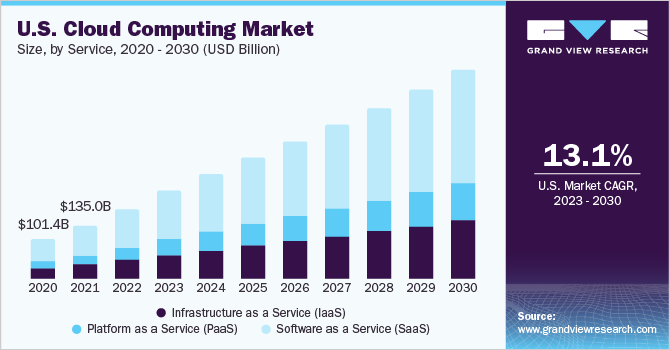
\includegraphics[scale=0.5]{Pictures/3_cloud_computing_market.png}
    \caption{U.S. cloud computing market\textsuperscript{\cite{market_cloud_computing}}.}
    \label{fig:3_cloud_computing_market}
\end{figure}

\section{Microservices}
This section of the thesis is dedicated to a comprehensive exploration of microservices as an
architectural choice that has seen an increasingly popularity over the past half-decade. It aims to
unpack the intricacies of microservices, given a broad overview of the core ideas behind this technology and some
reasons why these architectures are used so widely.

\subsection{Characteristics}
Microservices architecture is a modular approach to software development, breaking complex
applications into smaller, independent components—microservices—tailored to specific business
domains like inventory management or order processing. These microservices, with well-defined
interfaces, can be developed and deployed independently, ensuring flexibility and the evolution of
each component without affecting others. This architecture supports a service-oriented approach,
emphasizing independent deployability and technology neutrality, suitable for diverse technical
challenges\textsuperscript{\cite{microservices_book}}.
\newline\newline
Internally, microservices encapsulate their functionality, operating via network endpoints and
hiding implementation details like programming languages or data storage. This ensures effective
complexity management, with each service maintaining its own data storage, avoiding shared database
issues.
\newline\newline
Externally, microservices act as 'black boxes,' offering functionality without exposing internal
processes. This approach protects against impacts from internal changes, as long as interfaces
remain compatible. It enables seamless updates and maintenance, supporting independent development
and continuous integration.
\newline\newline
Key characteristics of microservices include loose coupling for flexibility and high cohesion for
maintainability. They allow targeted scalability, parallel team work, and robust security, with each
service secured separately. This makes microservices ideal for creating adaptable, scalable, and
sustainable software in rapidly evolving business and technology environments.

\subsubsection{Microservices in the Context of Cloud Computing}
The integration of microservices and cloud computing marks a significant progression in software
architecture, fostering dynamic, scalable, and resilient systems. The decentralized nature of
microservices aligns seamlessly with cloud environments, providing agility and scalable
infrastructure to meet varying service demands. Cloud platforms enhance resource optimization,
ensuring efficient and cost-effective operations. This synergy enables organizations to exploit
cloud computing's robustness, supporting microservices' complex interactions for heightened
scalability and resilience. It allows for continuous integration and deployment, promoting rapid
innovation. Additionally, strategic distribution of microservices across various regions in the
cloud enhances fault tolerance and ensures a consistent user experience globally.

\subsubsection{Example of a Microservice Architecture}
A prime example of microservices in action is the streaming giant Netflix, which has become
synonymous with the successful implementation of this architectural style. The backend architecture
of Netflix, a detailed account of which is provided in an article on
DEV.to\textsuperscript{\cite{microservice_example}}, is a testament to the company's innovative
engineering approach.

\begin{figure}
    \centering
    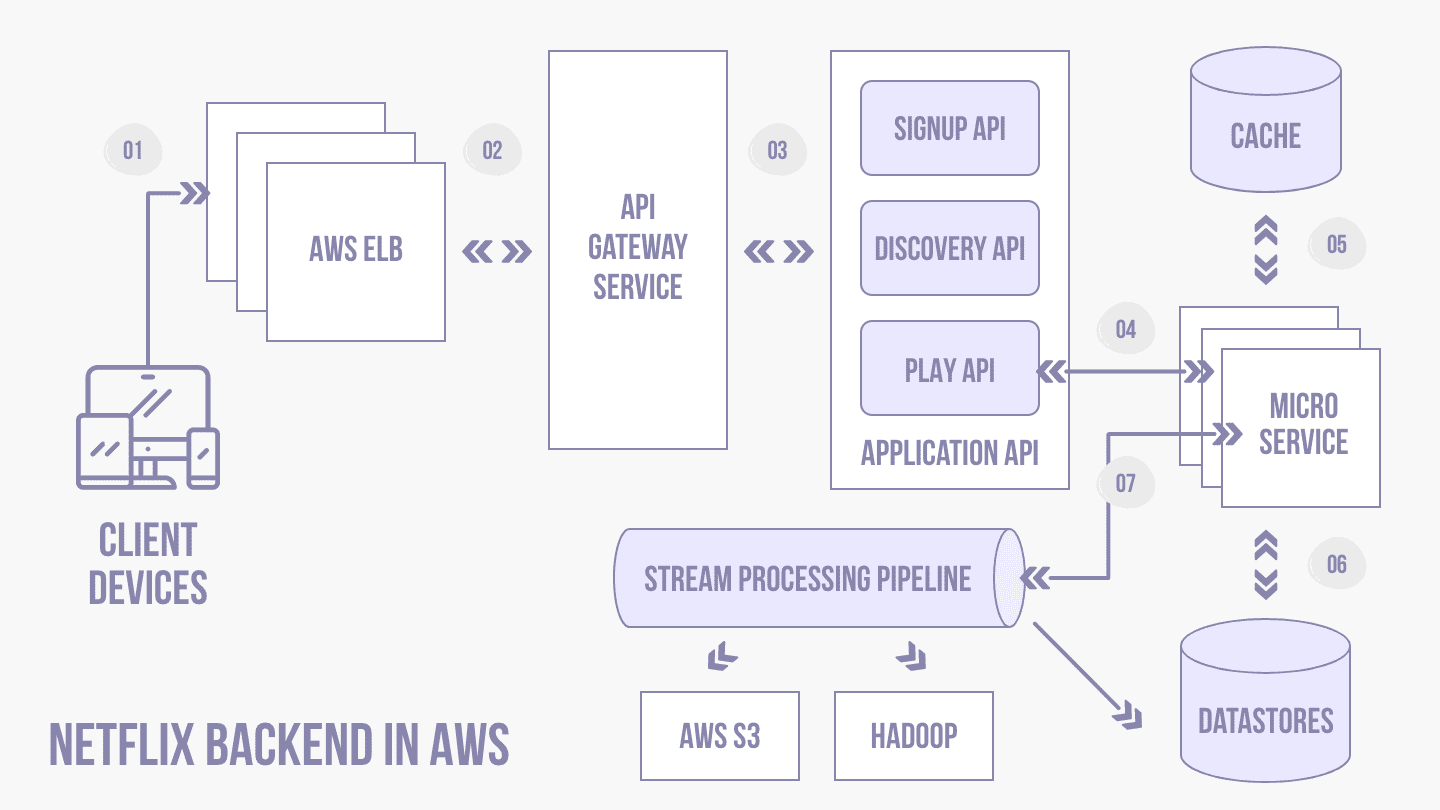
\includegraphics[scale=0.25]{Pictures/3_netflix.png}
    \caption{Netflix backend in AWS\textsuperscript{\cite{microservice_example_image}}.}
    \label{fig:3_netflix}
\end{figure}

How we can see in Figure \ref{fig:3_netflix}, Netflix's backend is a conglomeration of microservices
that operate on Amazon Web Services (AWS), enabling them to serve a staggering amount of content
globally with high availability and resilience. Each microservice is designed to perform a specific
function, such as handling login requests, processing user recommendations, or managing customer
support interactions. This division of responsibilities allows for independent scaling and
development of services, which is crucial given the diversity of Netflix's content and the
variability in demand. The microservices architecture is not only a core component of their backend
system but also underpins their Open Connect content delivery network (CDN), ensuring optimal
streaming performance by placing servers within Internet Service Provider (ISP) networks around the
world. This architecture facilitates rapid and reliable delivery of complex applications at scale,
illustrating the microservices model's capacity to support large-scale enterprise systems
efficiently and effectively.

\newpage

\subsection{Benefits}
This section delves into the multifaceted advantages of adopting microservices. From enhanced
scalability to independent deployment cycles, microservices promise a range of benefits that cater
to both technical and business needs. By dissecting these advantages, this section aims to elucidate
why microservices are becoming the architectural choice for many modern enterprises, providing them
with the flexibility and agility required to thrive in a competitive
market\textsuperscript{\cite{microservices_gitlab}}.

\subsubsection{Scalability}
Microservices excel in scalability due to their ability to be scaled individually. This granular
scalability allows for precise allocation of resources to different components based on fluctuating
demands, leading to enhanced efficiency in resource utilization. Unlike monolithic architectures,
where scaling often requires scaling the entire application, microservices operate independently.
This independence facilitates the seamless addition, removal, updating, or scaling of each service
without causing interruptions to the rest of the system. Organizations benefit from this by being
able to dynamically allocate resources to microservices experiencing spikes in demand—such as during
peak shopping seasons—and similarly, scale them down when demand wanes, thereby optimizing the use
of resources and computing power across the service landscape.

\subsubsection{Robustness}
Microservices architecture enhances the robustness of software applications by leveraging its
inherent decoupling. Individual services can fail without precipitating a system-wide shutdown,
thereby preventing a single point of failure from causing cascading breakdowns. In comparison,
monolithic architectures are susceptible to the domino effect, where a single component's failure
can paralyze the whole application. Microservices inherently design for failure, allowing the system
to degrade gracefully and maintain functionality even when certain services are down. However,
network and machine failures are inevitable, and strategies must be in place to handle these
incidents without significantly affecting the user experience.

\subsubsection{Technology agnostic}
Microservices architecture stands out for its technological flexibility, granting teams the liberty
to select the most suitable technology stack for each distinct service. This technology-agnostic
approach decouples services from any singular, early-stage technology decisions that often constrain
entire projects. Within this paradigm, each microservice can be developed using different
programming languages and data storage solutions, according to what best serves its purpose. This
not only streamlines development by aligning with teams' existing proficiencies but also avoids the
overhead of learning new languages unnecessarily. For instance, organizations like Netflix and
Twitter predominantly utilize the Java Virtual Machine (JVM) as their operational platform
\textsuperscript{\cite{microservices_book}}. Their choice is driven by a deep familiarity with this
technology.

\subsubsection{Distributed Development}
Microservices architecture allows development teams to independently build, deploy, and manage their
services, speeding up updates and feature additions with minimal disruption to the overall system.
This facilitates swift adaptation to changing business needs. Unlike monolithic applications, which
require large-scale deployments for minor updates, microservices support targeted, independent
changes to specific services. This reduces deployment risks, enables quick error recovery, and
hastens the delivery of new features to customers. Companies like Amazon and Netflix leverage
microservices to bypass obstacles in software delivery, ensuring rapid and reliable service to their
users\textsuperscript{\cite{microservices_book}}.

\subsubsection{Team optimization}
Microservices architecture enhances team productivity by adhering to the "two-pizza rule," where
smaller teams—ideally just large enough to be fed with two pizzas—tend to produce higher quality
outcomes due to improved focus and manageability. This approach, pioneered by Amazon, ensures that
each team works on a discrete codebase, fostering efficiency and faster achievement of goals. The
flexibility inherent in microservices also allows for easy reassignment of service ownership,
facilitating a seamless adaptation of the architecture to align with evolving organizational
structures, thereby maintaining efficiency and effectiveness in the long term.


\subsection{Challenges}
While the microservices architecture offers numerous benefits such as enhanced scalability and
improved team productivity, it also introduces a set of challenges that can complicate system design
and maintenance: the complexity of orchestrating numerous services, maintaining data consistency
across distributed systems and managing inter-service communication efficiently. Addressing these
challenges is essential for a smooth microservices architecture.

\subsubsection{Complexity}
The decentralized approach of microservices inherently leads to systems with a high degree of
complexity. As the number of services increases, the overall system can become more challenging to
oversee and manage. Debugging exemplifies this complexity; with each microservice generating its
logs, pinpointing the source of an issue can become a substantial challenge. This complexity
requires robust logging and monitoring solutions that can aggregate and correlate logs from across
services, providing a cohesive view of the system's health and facilitating faster problem
resolution. Additionally, the complexity demands that developers and operators have a clear
understanding of the system's architecture and communication patterns, ensuring they can effectively
trace and troubleshoot issues as they arise.

\subsubsection{Data Consistency}
Ensuring data consistency across microservices poses significant challenges due to their distributed
design. Unlike monolithic systems that rely on a single database, microservices often use separate
databases, making traditional transaction-based consistency difficult to maintain. As a result,
developers need to shift toward patterns like sagas and embrace eventual consistency, which can be a
major paradigm shift, especially when adapting existing systems. It's crucial to decompose
applications incrementally, allowing for careful evaluation of each change's impact on the system's
data integrity.

\subsubsection{Inter-service Communication}
In microservices architecture, especially in cloud environments, inter-service communication adds
complexity due to distributed network use. Each microservice's unique API requires careful
management to ensure compatibility, a significant task when hundreds or thousands of APIs are
involved. Disaggregating processes into multiple network-dependent services increases serialization,
transmission, and deserialization, potentially adding to latency. This impact on performance, hard
to predict in design or development, highlights the need for a gradual transition to microservices,
allowing for an assessment of changes on system latency.

\subsection{Comparison with Monolithic Architecture}

\begin{figure}
    \centering
    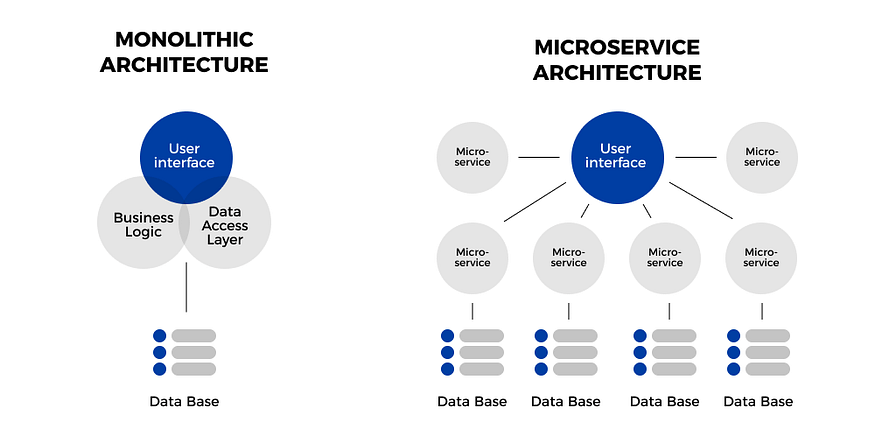
\includegraphics[scale=0.5]{Pictures/3_micro_mono.png}
    \caption{Monolithic and Microservices architectures\textsuperscript{\cite{monoliths_medium}}.}
    \label{fig:3_micro_mono}
\end{figure}

In Figure \ref{fig:3_micro_mono}, the distinction between a microservices approach and monolithic
architecture is illustrated. The latter is characterized by tightly coupled and interdependent
software components, any changes require building and deploying the entire stack, which can be slow
and error-prone. Microservices are designed to overcome these limitations by decomposing
functionality into separate services, each with a specific role, thus providing a more flexible and
scalable architecture. The table \ref{tab:micro_vs_mono} contains an overview of the differences
between the two approaches.

\begin{table}
    \centering
    \begin{tabular}{|l|p{5cm}|p{5cm}|}
        \hline
        \textbf{}            & \textbf{Monolithic}                                                                    & \textbf{Microservices}                                                       \\ \hline
        \textbf{Deployment}  & Simple and fast deployment of the entire system                                        & Requires distinct resources, making orchestrating the deployment complicated \\ \hline
        \textbf{Scalability} & It is hard to maintain and handle new changes; the whole system needs to be redeployed & Each element can be scaled independently without downtime                    \\ \hline
        \textbf{Agility}     & Not flexible and impossible to adopt new tech, languages, or frameworks                & Integrate with new technologies to solve business purposes                   \\ \hline
        \textbf{Resiliency}  & One bug or issue can affect the whole system                                           & A failure in one microservice does not affect other services                 \\ \hline
        \textbf{Testing}     & End-to-end testing                                                                     & Independent components need to be tested individually                        \\ \hline
        \textbf{Security}    & Communication within a single unit makes data processing secure                        & Interprocess communication requires API gateways raising security issues     \\ \hline
        \textbf{Development} & Impossible to distribute the team’s efforts due to the huge indivisible database       & A team of developers can work independently on each component                \\ \hline
    \end{tabular}
    \caption{Comparison of Monolithic and Microservices architectures\textsuperscript{\cite{monoliths_avenga}}.}
    \label{tab:micro_vs_mono}
\end{table}

\section{How to Model Microservices}
This section is dedicated to exploring key principles such as information hiding, coupling, and
cohesion, which are crucial in shaping our approach to defining the limits of our microservices. We
will place a particular focus on domain-driven design, a highly effective strategy that plays a
crucial role in establishing the boundaries of your microservices. This approach not only maximizes
their advantages but also effectively reduces potential risks.

\subsection{Boundaries}
Our goal is to design microservices that can be independently modified, deployed, and have their
features released to users without relying on others. The ability to update a single microservice
independently from the others is crucial. At their core, microservices represent a type of modular
decomposition, but with network interactions between modules. This means we can rely on a lot of
prior art in the space of modular software to assist in defining our boundaries. Bearing this in
mind, we will delve into three essential concepts crucial for identifying effective microservice
boundaries: information hiding, cohesion, and coupling\textsuperscript{\cite{microservices_book}}.

\subsubsection{Information Hiding}
Information hiding is a concept developed by David Parnas to look at the most effective way to
define module boundaries\textsuperscript{\cite{microservices_model_1}}. Information hiding aims to
conceal as much detail as possible within a microservice boundary. Parnas
write\textsuperscript{\cite{microservices_model_2}}:

\begin{quote}
    The connections between modules are the assumptions which the modules make about each other.
\end{quote}

Reducing assumptions between modules in microservices simplifies their connections, making it easier
to modify one module without affecting others. This approach also allows developers to make safer
changes, as they understand how their module is used by others, preventing the need for changes in
upstream components. Additionally, in microservices, such modifications can be deployed
independently, enhancing the benefits outlined by Parnas: faster development, better
comprehensibility, and increased flexibility.

% \begin{itemize}
%     \item \textbf{Improved development time}: Enabling independent development of modules
%           facilitates parallel work, thus diminishing the complexities often associated with increasing
%           the number of developers on a project.
%     \item \textbf{Comprehensibility}: The ability to examine and comprehend each module separately
%           simplifies the process of grasping the system’s overall functionality.
%     \item \textbf{Flexibility}: The independence of modules allows for alterations in one without
%           necessitating changes in others. Furthermore, this independence provides the flexibility to
%           recombine modules in various configurations, creating new functionalities.
% \end{itemize}

\subsubsection{Coupling and Cohesion}
The concepts of coupling and cohesion are integral to the structure and stability of microservice
architectures. Understanding their interplay helps in designing systems that are both stable and
efficient.
% Cohesion refers to how closely related the functionalities within a microservice are,
% aiming for a strong internal unity. Coupling, on the other hand, deals with the degree of
% interdependence between different microservices, where the goal is to minimize dependencies to
% achieve loose coupling. 
Achieving the right balance between these two aspects is crucial for the
effective functioning of microservices.

\begin{itemize}
    \item \textbf{Cohesion}: Cohesion in microservices is about strategically grouping related
          business functionalities to reduce the need for changes across multiple areas. It emphasizes
          consolidating similar behaviors in a single location, which streamlines the process of
          modification and deployment. This approach leads to strong cohesion, where closely related
          functionalities are contained within a single microservice, thereby enabling faster and more
          secure updates and changes.
    \item \textbf{Coupling}: Coupling in the context of microservices involves designing services in
          a way that changes in one do not require modifications in others. This design principle promotes
          minimal inter-service knowledge, thereby reducing dependencies between different services. The
          ideal state of loose coupling is achieved when services have minimal interactions with each
          other, maintaining their independence. This approach significantly reduces the risks associated
          with tightly interconnected systems, ensuring more robust and flexible service architecture.
\end{itemize}

This balance is not only about the technical aspects but also about making pragmatic decisions that
fit the specific context and challenges of the project.

\subsubsection{Types of Coupling}
The concept of coupling in system design is nuanced and not as straightforward as it might initially
appear. While it's true that excessive coupling can lead to various challenges in system
architecture, some level of coupling is inevitable and, in certain cases, necessary. The key
objective in effective system design is not to eliminate coupling entirely but to manage and
minimize its extent.

\begin{figure}
    \centering
    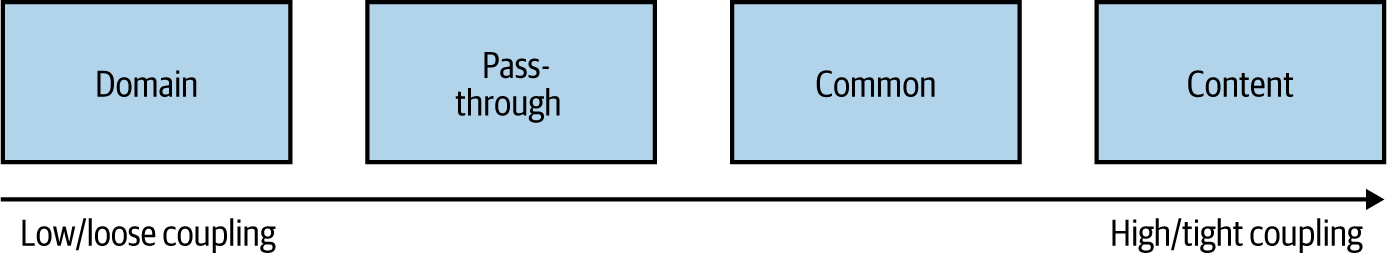
\includegraphics[scale=0.5]{Pictures/3_types_coupling.png}
    \caption{The different types of coupling, from loose (low) to tight (high)}.
    \label{fig:3_types_coupling}
\end{figure}

The different types of coupling\textsuperscript{\cite{microservices_book}}, as depicted in Figure
\ref{fig:3_types_coupling}, provide a comprehensive spectrum, ranging from low to high. Low coupling
is generally desirable as it indicates a system where components operate independently, enhancing
flexibility and ease of maintenance. High coupling, on the other hand, suggests a tightly
interlinked system where changes in one component can have significant ripple effects, making it
less desirable due to the increased complexity and risk involved. Understanding these variations and
their implications is crucial for designing robust, scalable, and maintainable systems.

\begin{itemize}
    \item \textbf{Domain Coupling}: Domain coupling refers to a scenario where one microservice
          depends on another for specific functionalities. While such interactions are largely inevitable
          in a microservice architecture, where collaboration among multiple services is essential for
          system operation, it's important to minimize these interactions. It is a form
          of loose coupling in microservices, but can lead to issues if a service relies too heavily on many
          downstream services, suggesting over-centralization of logic. Problems may also arise from
          exchanging complex data sets between services. It's advisable to share only essential
          information and minimize data exchange.
    \item \textbf{Pass-Through Coupling}: Pass-through coupling in microservices occurs when one
          microservice transmits data to another solely for the use of a subsequent downstream service.
          This form of coupling is particularly challenging within implementation strategies, as it
          suggests that the initiating service is aware not only of the direct recipient microservice but
          may also need to understand the functioning of the microservice further down the chain. This
          creates a complex interdependency where knowledge of multiple services and their interactions
          becomes necessary, complicating the architecture.
    \item \textbf{Common Coupling}: Common coupling in microservices refers to the scenario where
          multiple services utilize the same data set, such as a shared database, memory, or filesystem.
          This coupling becomes problematic when changes to the data's structure affect several services
          simultaneously. For example, if the schema of a commonly used database changes incompatibly, all
          services relying on it need updates. Additionally, common coupling can lead to resource
          contention issues, as multiple services accessing the same database or filesystem may strain or
          even incapacitate that resource. While sometimes manageable, common coupling often indicates a
          lack of cohesion in the system and can pose operational challenges, making it one of the less
          desirable forms of coupling.
    \item \textbf{Content Coupling}: Content coupling occurs when an upstream service intrusively
          modifies the internal state of a downstream service, commonly by directly accessing and altering
          the latter's database. This is subtly different from common coupling, where multiple services
          interact with a shared dataset, but acknowledge it as an external, uncontrollable dependency.
          Content coupling blurs ownership lines, complicating system modifications for developers. A
          clear distinction in microservices between changeable and unchangeable elements is crucial.
          Developers must be aware of the service contract exposed to external parties to avoid disrupting
          upstream consumers. While common coupling shares some issues with content coupling, the latter
          introduces additional complexities, often termed pathological coupling. Direct external access
          to a database challenges the definition of what can be safely altered and what cannot,
          undermining the principle of information hiding. Therefore, content coupling is best avoided due
          to these inherent complications.
\end{itemize}

% volendo puoi mettere le immagini

\subsection{Domain-Driven Design}
In defining microservice boundaries, we primarily focus on the domain itself, applying domain-driven
design (DDD) to model our domain more effectively. DDD, as introduced by Eric Evans in
"Domain-Driven Design"\textsuperscript{\cite{ddd_book}}, provides key concepts that are crucial in
this context. These include Ubiquitous Language, which ensures uniform language usage across the
domain; Aggregates, which group related domain objects into a single unit; and Bounded Context,
which sets the scope of applicability for a particular model. These principles play a vital role in
guiding our microservice architecture strategy.

\subsubsection{Ubiquitous Language}
Ubiquitous language emphasizes the importance of aligning the terminology in our code with the terms
used by the users. This commonality of language between the development team and the end users
simplifies modeling the real-world domain and enhances communication. Integrating real-world
language into the code streamlines the development process. It allows developers, when handling
tasks or stories, to quickly grasp the requirements and objectives, as these are expressed in terms
familiar to both the product owner and the development team.

\subsubsection{Aggregates}
Aggregates in microservice architecture are envisioned as self-contained units, each with its own
state, identity, and life cycle that mirrors real-world entities. These aggregates are apt for
implementation as state machines, given their inherent life cycles. The design focuses on
consolidating the code that manages state transitions with the aggregate's state itself. Typically,
a single microservice is responsible for one aggregate, but it may handle several. For instance, an
Invoice aggregate would include various line payments, each significant only within the context of
the overall Invoice aggregate.
\newline\newline
A microservice's role extends to managing the life cycle and data storage of one or several types of
aggregates. Should a different service need to modify an aggregate, it must either directly request
this change or prompt the aggregate to initiate its own state transitions, possibly in response to
events from other microservices. Aggregates are designed with the capability to reject inappropriate
state transition requests, underscoring the importance of preventing illegal state changes in their
implementation.

\subsubsection{Bounded Context}
A bounded context usually reflects a larger section of an organization, with clear responsibilities
within its boundaries. This concept focuses on concealing the finer details of implementation,
safeguarding internal aspects that aren't necessary for external understanding or involvement.
\newline\newline
In terms of structure, a bounded context comprises one or more aggregates. While some of these
aggregates might be visible externally, others remain internal to maintain the integrity of the
context. Bounded contexts can also form relationships with other contexts, translating into
dependencies between services in a microservice architecture.
\newline\newline
For instance, a warehouse service can be seen as a bounded context, bustling with activities like
processing outgoing orders, receiving new inventory, and other logistical tasks. In a different
bounded context, such as the finance department, the focus shifts to less dynamic but equally vital
functions like managing payroll and handling financial transactions. Each context operates within
its own realm of responsibilities but may interact with or depend on other contexts, reflecting the
interconnected nature of services in a microservices setup.

\subsubsection{Domain-Driven Design in Microservices}
Domain-Driven Design (DDD) is effective in microservices architecture due to its focus on bounded
contexts which conceal internal complexities and present clear boundaries to the system. These
contexts aid in maintaining stable microservice boundaries by ensuring that internal changes do not
affect other system parts. When systems are segmented along bounded contexts, modifications for
business needs are confined to specific microservices, streamlining deployment and reducing the
complexity of changes.

\newpage

\begin{figure}
    \centering
    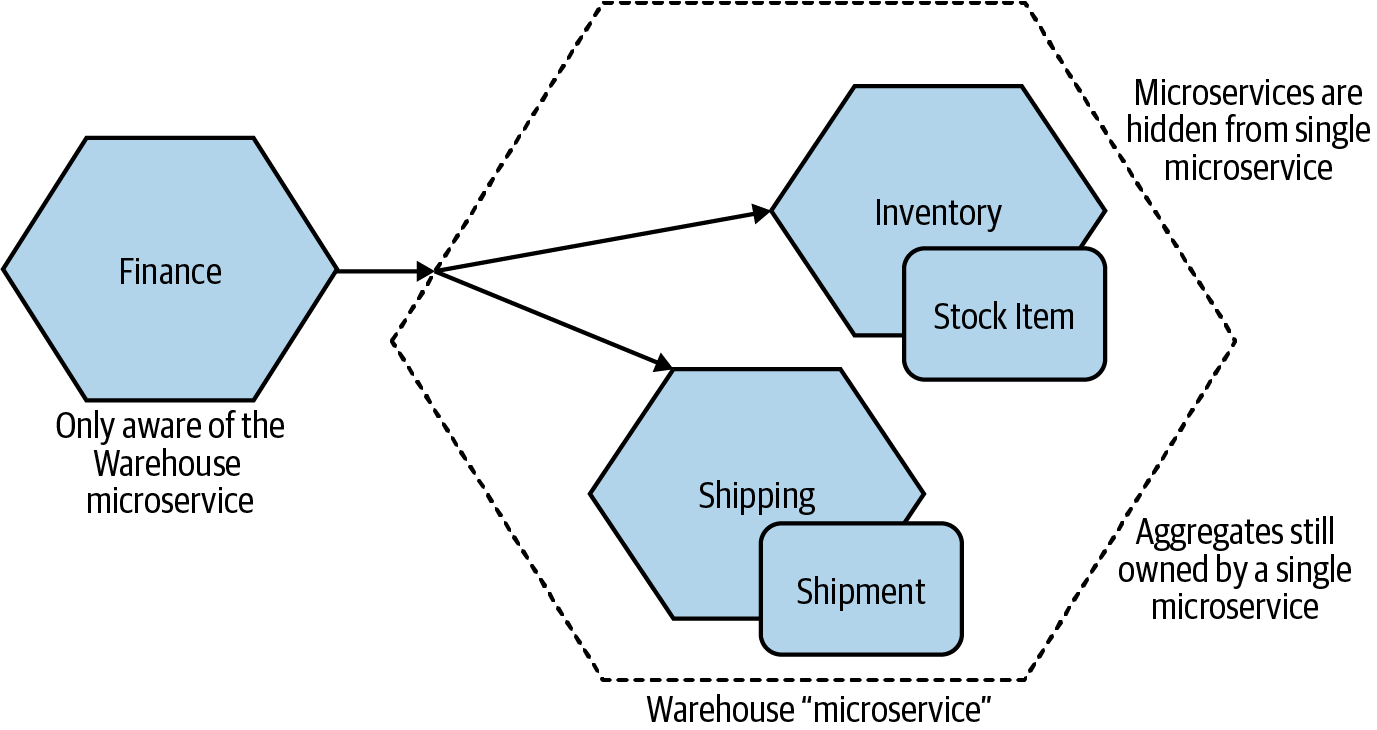
\includegraphics[scale=0.5]{Pictures/3_ddd.png}
    \caption{The Warehouse service internally has been split into Inventory and Shipping microservices}.
    \label{fig:3_ddd}
\end{figure}

Aggregates and bounded contexts both provide cohesive units with clear interfaces to the larger
system. Aggregates are focused state machines for single domain concepts, while bounded contexts
group these aggregates and represent them to the outside world. These constructs are ideal for
defining microservice boundaries. Initially, it's beneficial to work with services that cover
complete bounded contexts. If needed, services can later be divided into smaller ones without
splitting individual aggregates, keeping such internal decisions invisible to external stakeholders.
For instance, a Warehouse service may internally be divided into Inventory and Shipping, but
externally it remains a singular Warehouse microservice to users, as depicted in the figure
\ref{fig:3_ddd}.

\subsection{Coordination Management}
In the environment of microservices, the complexity of interactions extends beyond the simple
communication between two services. A critical aspect is the orchestration of multiple microservices
working together to execute comprehensive business processes. This orchestration requires a nuanced
approach to maintain the system's integrity and efficiency.
\newline\newline
In this section, we'll explore how microservices can collaborate on workflows and processes. We'll
delve into strategies like distributed transactions, which attempt to address these coordination
challenges, and examine the saga pattern, an advanced concept that provides a structured approach to
manage long-running, distributed business transactions within microservice architectures.

\subsubsection{Database Transactions}
In computing, transactions are a series of actions completed as a single unit, ensuring all changes
are made or none if an error occurs. This concept is crucial in databases, where transactions (like
insertions, deletions, or updates) must be successful, often spanning multiple tables. The term
database transactions usually refers to ACID transactions\textsuperscript{\cite{microservice_acid}},
which is explained in table \ref{tab:acid}.

\begin{table}
    \centering
    \begin{tabular}{|c|l|p{0.6\linewidth}|}
        \hline
        \textbf{Letter} & \textbf{Stands for} & \textbf{Description}                                                                             \\ \hline
        A               & Atomicity           & Ensures that all parts of a transaction are completed successfully, or none at all.              \\ \hline
        C               & Consistency         & Guarantees that a transaction only brings the system from one valid state to another.            \\ \hline
        I               & Isolation           & Ensures that transactions are performed independently and transparently.                         \\ \hline
        D               & Durability          & Assures that once a transaction is committed, it will remain so, even in the event of a failure. \\ \hline
    \end{tabular}
    \caption{ACID properties of database transactions}
    \label{tab:acid}
\end{table}

In microservices, ACID transactions apply to local operations within a single microservice,
complicating atomic operations across multiple services. Unlike a monolithic database that ensures
atomicity through ACID properties, a distributed microservices system handles changes across
separate databases, as depicted in Figure \ref{fig:3_transaction}. This leads to independent
transactions that may succeed or fail separately, lacking atomicity for the entire operation.

% When it comes to microservices, the use of ACID transactions still applies, but their scope is
% confined to the local operations within an individual microservice. This presents a challenge, as
% the atomicity of operations across multiple microservices is not inherently guaranteed. For
% instance, an operation that changes a customer's status and removes them from a "PendingEnrollments"
% table is straightforward in a monolithic single database environment due to the ACID properties.
% However, as shown in Figure \ref{fig:3_transaction}, in a distributed microservices setup these
% changes are split across different databases and hence become two distinct transactions. This
% separation means that we may no longer have the atomicity of the entire operation, as each
% transaction may succeed or fail independently.

\begin{figure}
    \centering
    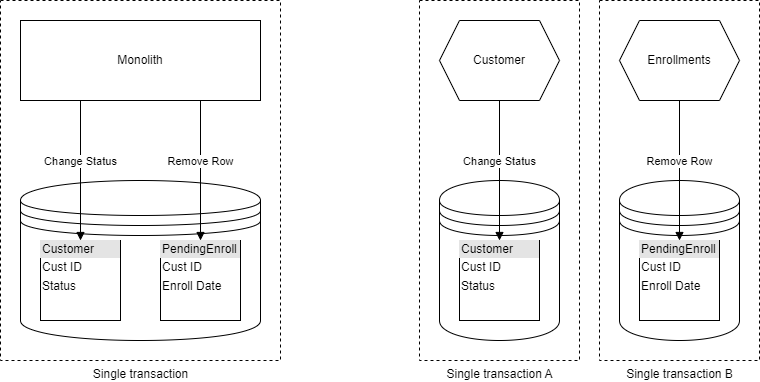
\includegraphics[scale=0.5]{Pictures/3_transaction.png}
    \caption{Example that show the difference between monolithic and microservices transactions.}
    \label{fig:3_transaction}
\end{figure}

\subsubsection{Distributed transaction - Two-Phase Commit}
The Two-Phase Commit (2PC) algorithm facilitates transactional updates across distributed systems,
ensuring atomic transaction commits across multiple nodes. Essentially, it mandates that all
involved nodes must either commit or abort together, maintaining the principle of atomic
transactions\textsuperscript{\cite{2pc_1}}. Unfortunately, 2PC is often viewed as impractical for
microservice architectures\textsuperscript{\cite{microservices_book}}, thus this section explores the
reasons behind this perspective, analyzing the limitations and challenges of applying 2PC in such
contexts.

\begin{figure}
    \centering
    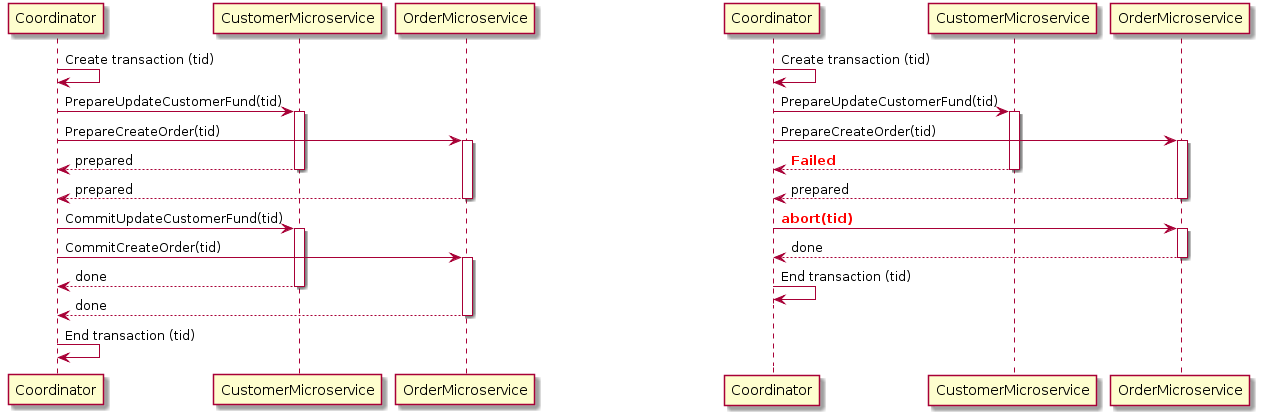
\includegraphics[scale=0.55]{Pictures/3_2pc.png}
    \caption{Example of the 2PC protocol process\textsuperscript{\cite{2pc_2}}.}
    \label{fig:3_2pc}
\end{figure}

In the figure \ref{fig:3_2pc} we can see an example of the 2PC protocol process. The protocol is divided
into two phases: the prepare phase and the commit phase. Initially, in the prepare phase,
microservices are prompted to ready themselves for a potential atomic data change. Following this,
the commit phase involves directing these microservices to execute the actual changes. Central to
this process is a global coordinator, responsible for overseeing the transaction's lifecycle and
engaging with microservices during both the prepare and commit phases. This coordinator is pivotal
in determining whether the nodes can commit the proposed transaction and in issuing the final
command to commit or abort\textsuperscript{\cite{2pc_1}}\textsuperscript{\cite{2pc_2}}.
\newline\newline
The major benefit of 2PC protocol is that it is a robust mechanism for ensuring consistency across
distributed systems. Its dual phases — prepare and commit — assure that transactions are atomic,
making all microservices commit successfully or none at all, preventing partial updates.
Additionally, 2PC enforces read-write isolation, ensuring that any modifications remain invisible
until the coordinating node finalizes the commit, maintaining transaction integrity throughout the
process\textsuperscript{\cite{2pc_2}}.
\newline\newline
Although 2PC ensures atomicity, its limitations make it less suitable for numerous
microservice-based systems\textsuperscript{\cite{2pc_2}}. The main issue of 2pc protocol
are\textsuperscript{\cite{2pc_3}}:

\begin{itemize}
    \item \textbf{Blocking}: The protocol locks objects until a transaction is complete, causing
          potential delays and deadlock.
    \item \textbf{Latency}: Waiting for all participant responses before proceeding adds to the
          transaction time.
    \item \textbf{Coordinator Risk}: The Transaction Coordinator is a critical point that can fail,
          blocking all transactions.
    \item \textbf{Participant Performance}: The entire transaction's speed is tied to the slowest
          participant, with failures necessitating full rollbacks.
\end{itemize}

\subsubsection{Saga distributed transactions pattern}
As described so far, to avoid coupling between microservices, the database-per-microservice pattern
is utilized, allowing each service to manage its own data. This method offers several advantages:
select the most suitable data store type, scale it independently, and maintain isolation from
failures in other services\textsuperscript{\cite{ms_sagas}}. This pattern has a drawback: it does
not support ACID transactions across multiple services. To overcome this limitation, the Saga
pattern can be employed.
\newline\newline
Unlike a two-phase commit, the saga pattern is designed to effectively coordinate multiple state
changes, ensuring data consistency and avoiding resource locks across microservices. It accomplishes
this by decomposing the process into separate, independently executable activities. The adoption of
the saga pattern necessitates the explicit modeling of business processes, which can yield
significant benefits\textsuperscript{\cite{microservices_book}}.

\begin{figure}
    \centering
    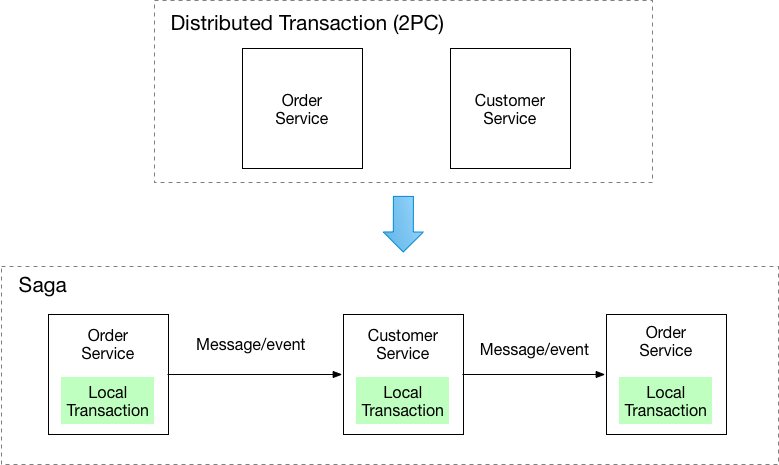
\includegraphics[scale=0.5]{Pictures/3_saga.png}
    \caption{From 2pc to Saga pattern\textsuperscript{\cite{io_sagas}}.}
    \label{fig:3_saga}
\end{figure}

How showed in figure \ref{fig:3_saga}, the Saga pattern manages transactions across multiple
services through a sequence of local transactions, each serving as an atomic work effort by a saga
participant. In this pattern, every local transaction updates the database and publishes a message
or event to initiate the subsequent local transaction within the saga. If any local transaction
fails, typically due to a violation of business rules, the saga responds by executing compensating
transactions to reverse the changes made by earlier local transactions. This approach ensures
consistent and reliable transaction management in complex, distributed
systems\textsuperscript{\cite{ms_sagas}}\textsuperscript{\cite{io_sagas}}.
\newline\newline
The key benefit of Saga is maintaining data consistency across multiple services without needing
distributed transactions. However, it introduces complexities: developers must create compensating
transactions to reverse earlier changes, and debugging becomes challenging, especially as the number
of services involved increases.
When a client initiates a saga through a synchronous request (like an HTTP POST), determining the
saga's outcome is crucial. This can be managed in several ways\textsuperscript{\cite{io_sagas}}:

\begin{itemize}
    \item \textbf{Immediate Response Post-Completion}: The service responds after the saga
          completes, ensuring a definitive outcome but possibly causing delays.
    \item \textbf{Initiation Acknowledgement with Periodic Polling}: The service acknowledges the
          saga's start, and the client periodically checks for the outcome.
    \item \textbf{Initiation Acknowledgement with Event Notification}: The service sends an initial
          response and notifies the client via an event (e.g., websocket) upon saga completion.
\end{itemize}

There are two prevalent methods for implementing the Saga pattern: choreography and orchestration.
Each method presents unique challenges and requires specific technologies to effectively coordinate
the workflow.

\subsubsection{Choreography-based saga}
Choreography in sagas refers to a decentralized method of coordination where participants
communicate through the exchange of events, without relying on a central control point. In this
approach, each local transaction emits domain events that activate local transactions in
other services\textsuperscript{\cite{ms_sagas}}.

\newpage

\begin{figure}
    \centering
    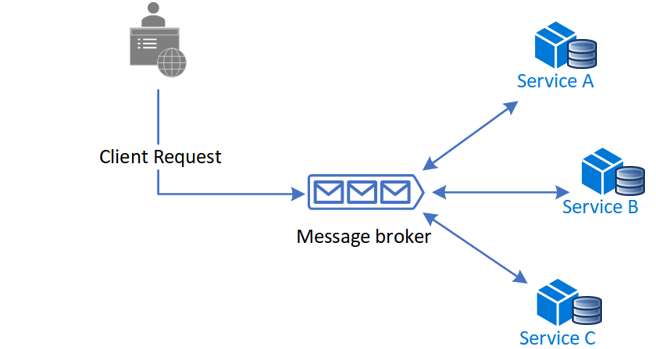
\includegraphics[scale=0.55]{Pictures/3_choreography.png}
    \caption{Choreography-based saga\textsuperscript{\cite{ms_sagas}}.}
    \label{fig:3_choreography}
\end{figure}

The workflow is well-suited for simpler processes with fewer participants, as it does not
necessitate complex coordination logic or the implementation and maintenance of an additional
service. This decentralization also prevents the emergence of a single point of failure. However,
the approach has its limitations; as the workflow grows, it becomes increasingly challenging to
track the interactions and commands between saga participants, potentially leading to cyclic
dependencies. Integration testing can be complicated, requiring all services to be
active to effectively simulate a transaction, posing a considerable challenge in practical
applications\textsuperscript{\cite{ms_sagas}}.

\subsubsection{Orchestration-based saga}
Orchestration in sagas involves a central controller directing saga participants on which local
transactions to carry out. The orchestrator manages all transactions, instructing participants on
specific operations in response to events. It is responsible for executing saga requests,
maintaining and interpreting the state of each task, and managing failure recovery through
compensating transactions\textsuperscript{\cite{ms_sagas}}.

\begin{figure}
    \centering
    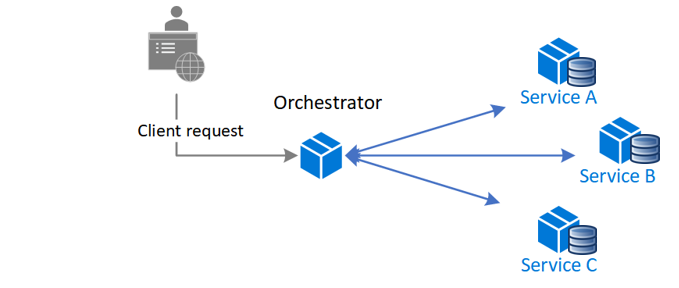
\includegraphics[scale=0.55]{Pictures/3_orchestrator.png}
    \caption{Orchestration-based saga\textsuperscript{\cite{ms_sagas}}.}
    \label{fig:3_orchestration}
\end{figure}

This pattern is advantageous for complex workflows with numerous participants or when incorporating
new participants over time, as it allows complete control over each participant and their
activities. This approach eliminates cyclical dependencies by having the orchestrator solely depend
on the saga participants and simplifies business logic by clearly separating concerns. Anyway, it
introduces additional design complexities by requiring the implementation of specific coordination
logic, and the orchestrator itself becomes a potential point of failure, managing the entire
workflow and thus presenting a risk to the system's stability\textsuperscript{\cite{ms_sagas}}.

\section{Serverless}
\subsection{Event-driven design}

\section{Technologies}
\subsection{Amazon AWS Services}
% https://aws.amazon.com/what-is-aws/
AWS is recognized as the world's most comprehensive and broadly adopted cloud platform. It offers
over 175 fully featured services from data centers globally. AWS is utilized by a diverse range of
customers, including rapidly growing startups, large enterprises, and leading government agencies,
to reduce costs, increase agility, and accelerate innovation. The platform provides a wide array of
cloud-based products including compute, storage, databases, analytics, networking, mobile, developer
tools, management tools, IoT, security, and enterprise applications, all available on-demand with
pay-as-you-go pricing.
\subsubsection{AWS API Gateway}
\subsubsection{AWS Lambda}
\subsubsection{AWS RDS}
\subsubsection{AWS SQS}
\subsubsection{AWS SNS}
\subsection{Firebase}
\subsection{GO Language}
\subsubsection{GO CDK}
\subsubsection{GORM}
\subsection{Serverless framework}
\subsection{Flutter}

\chapter{Technologies}
This chapter focuses on the specific technologies utilized in implementing Kube. Foremost among
these is the suite of AWS services, including Lambda for serverless computing, SQS (Simple Queue
Service) and SNS (Simple Notification Service) for messaging, and RDS (Relational Database Service)
for database management. These services collectively provide a resilient and scalable infrastructure
for Kube. Additionally, the platform leverages the serverless architecture to optimize resource
utilization and reduce operational overhead and the Go programming language for its efficiency and
suitability for building high-performance applications. The user interface of Kube is crafted using
Flutter, a versatile UI toolkit, which enhances the platform's accessibility and aesthetic appeal.
Together, these technologies form the cornerstone of Kube, enabling it to deliver good performance
and user experience.

\section{Amazon AWS Services}
AWS is recognized as the world's most comprehensive and broadly adopted cloud platform. It offers
over 175 fully featured services from data centers globally. AWS is utilized by a diverse range of
customers, including rapidly growing startups, large enterprises, and leading government agencies,
to reduce costs, increase agility, and accelerate innovation. The platform provides a wide array of
cloud-based products including compute, storage, databases, analytics, networking, mobile, developer
tools, management tools, IoT, security, and enterprise applications, all available on-demand with
pay-as-you-go pricing\textsuperscript{\cite{tech_1}}. In this section we will analyze the most
important services offered by Amazon AWS that we will use in the development of the project.

\newpage

\subsubsection{Example of AWS services integration}

\begin{figure}
    \centering
    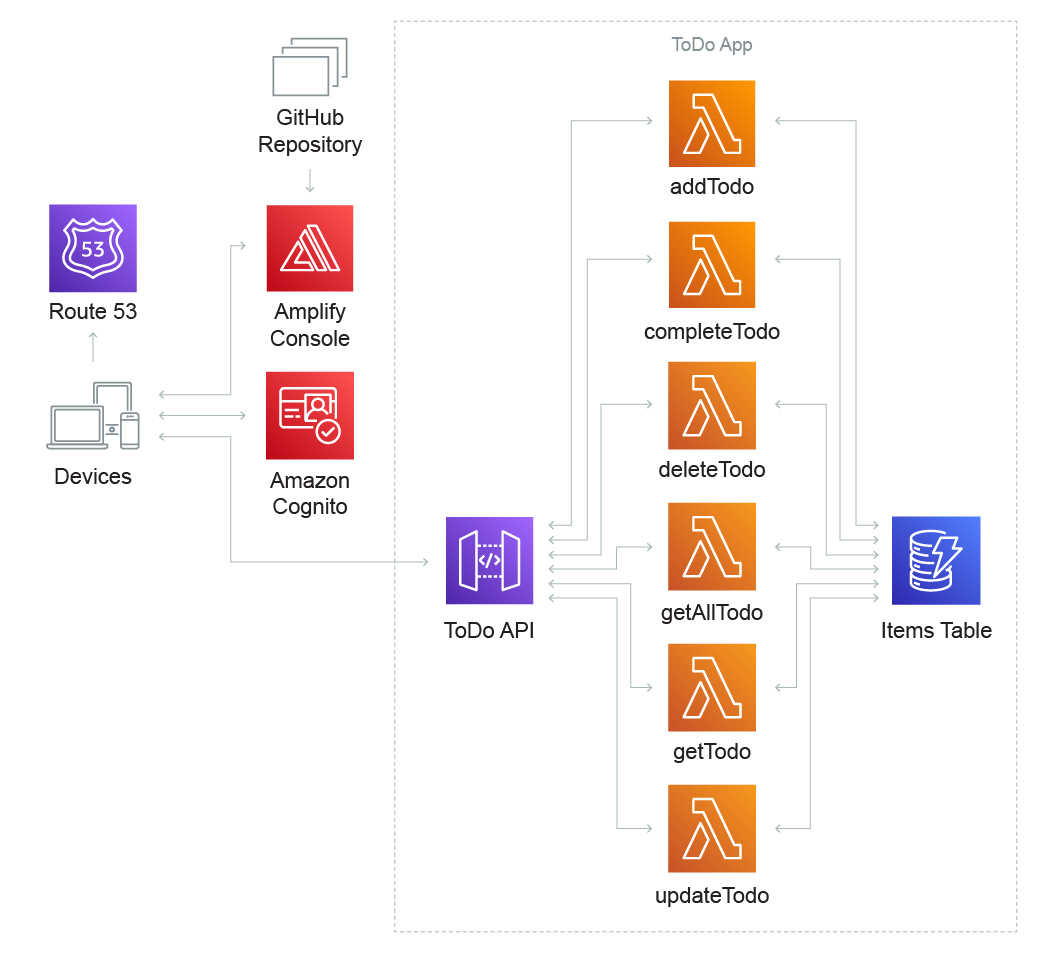
\includegraphics[scale=0.3]{Pictures/3_serverless_example.jpg}
    \caption{Example of AWS services integration.}
    \label{fig:3_aws_example}
\end{figure}

The image \ref{fig:3_aws_example} illustrates the architecture of a simple "to-do list" web
application built using serverless technology on the Amazon public cloud. This event-driven
application is designed to allow registered users to manage their tasks efficiently. Users interact
with the application to create, update, view, and delete to-do items. The architecture integrates
several Amazon Web Services to achieve this functionality. Each component of the architecture is
orchestrated to respond to specific events triggered by user actions, such as adding a new to-do
item or marking one as complete, making the entire application responsive and scalable without the
need to manage server infrastructure\textsuperscript{\cite{serverless_1}}.

\subsection{Pros and cons}
Amazon Web Services (AWS) is renowned for its extensive array of over 200 fully-featured services,
ranging from fundamental infrastructure technologies like compute, storage, and databases to
cutting-edge fields such as machine learning, AI, data lakes, analytics, and IoT. This diversity
offers tailored solutions for different applications, optimizing both cost and performance. However,
the sheer breadth of services can be overwhelming for less experienced users and creates a potential
dependency on AWS, making it challenging to switch providers. Additionally, while AWS allows for
cost and performance flexibility, improper resource management or unsuitable service choices can
lead to high expenses.

\subsection{Alternatives}
Microsoft Azure and Google Cloud Platform (GCP) stand as significant alternatives to Amazon Web
Services. Azure, backed by Microsoft's legacy in enterprise software, excels in integrating with
existing Windows-based environments, making it a preferred choice for organizations deeply embedded
in Microsoft's ecosystem. It offers a strong focus on hybrid cloud, AI, and machine learning
capabilities. On the other hand, GCP is highly regarded for its deep expertise in data analytics,
machine learning, and open source technologies, leveraging Google's pioneering work in these
areas\textsuperscript{\cite{cloud_azure}}\textsuperscript{\cite{cloud_google}}. The table
\ref{fig:3_cloud_comparision} shows a comparison between the major four cloud services providers.

\begin{figure}
    \centering
    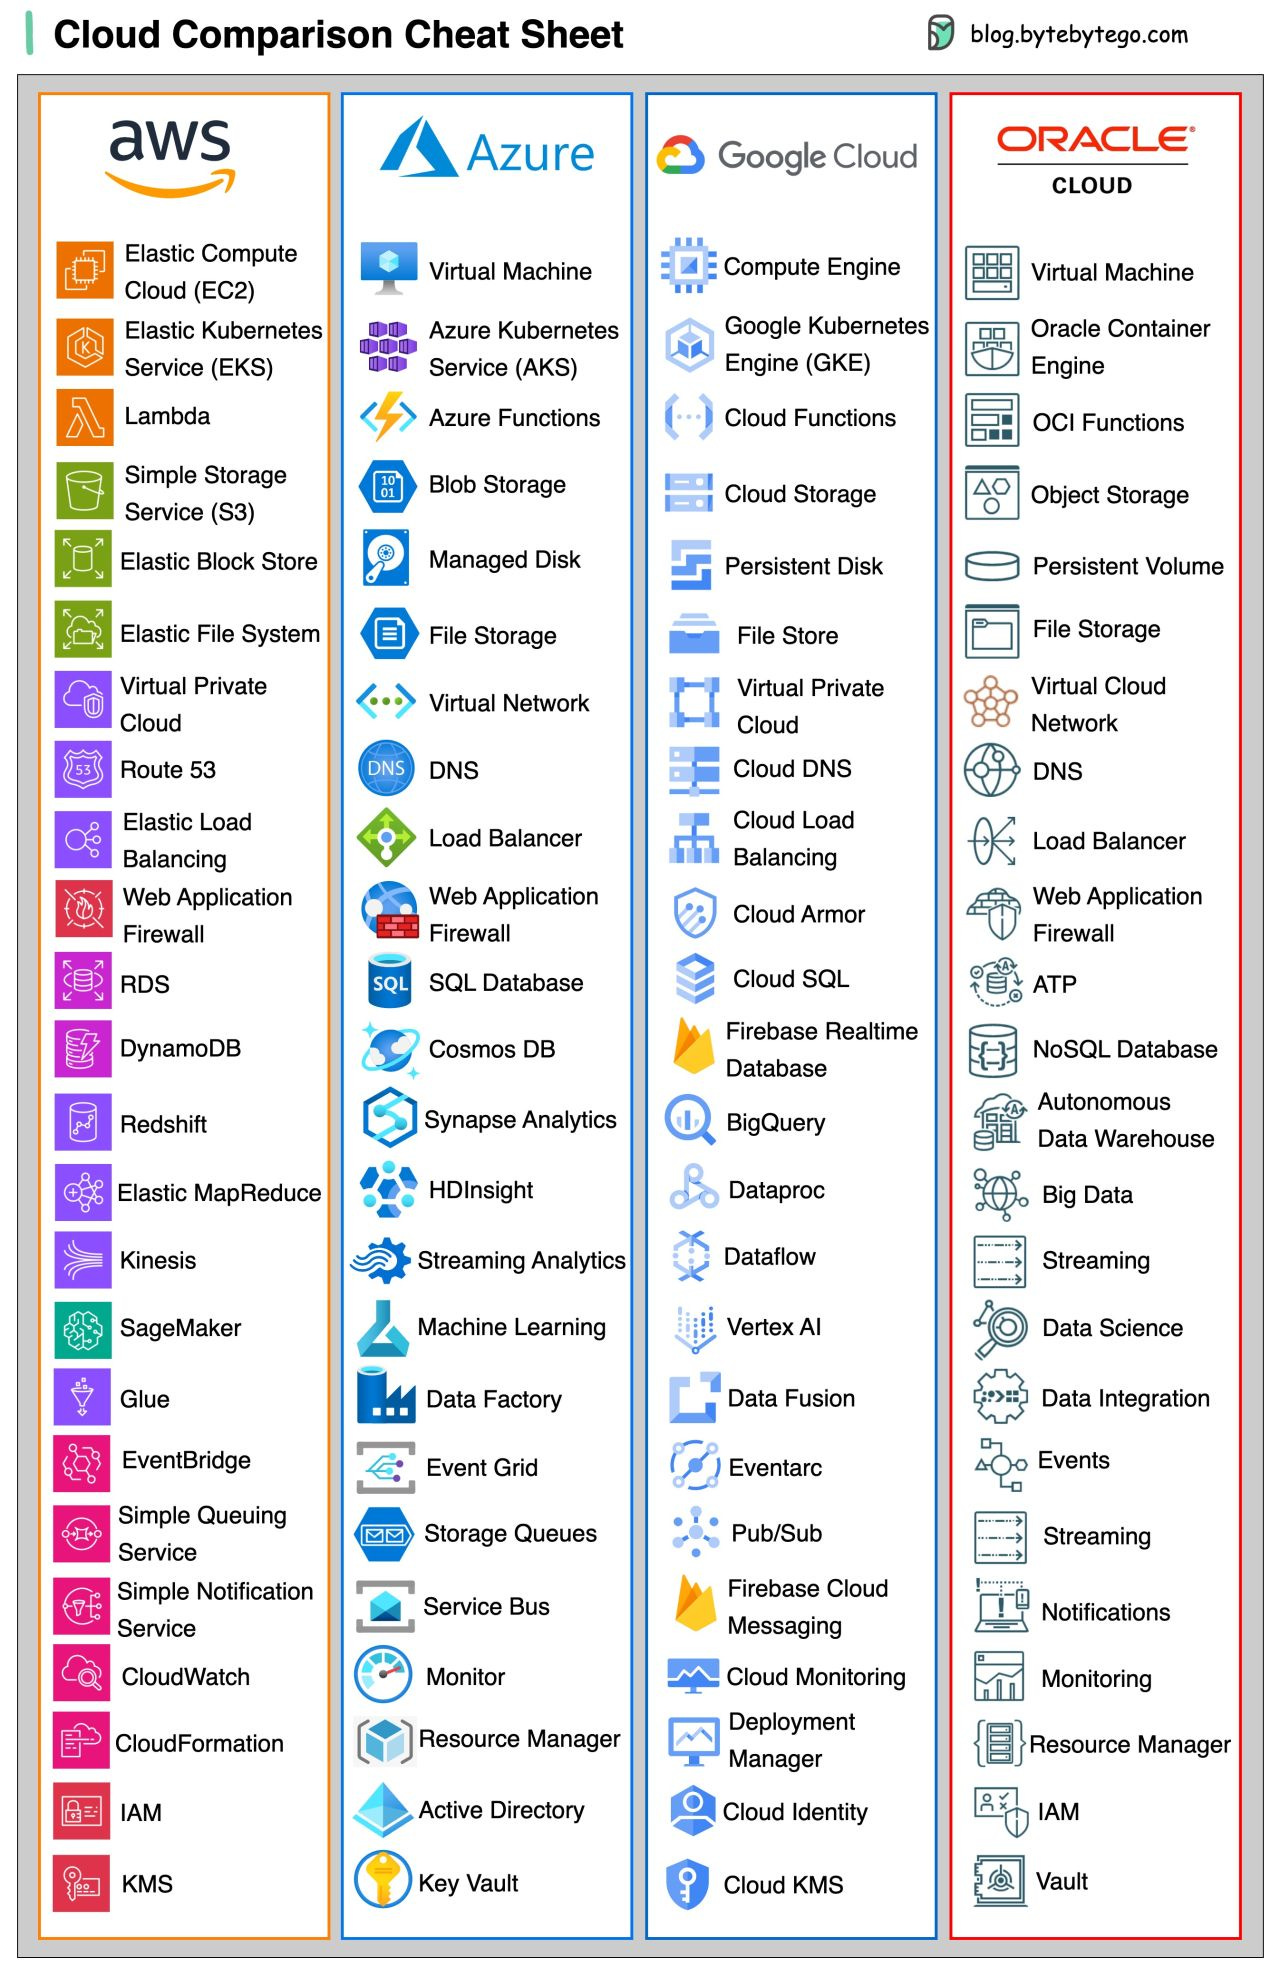
\includegraphics[scale=0.18]{Pictures/3_cloud_comparision.jpg}
    \caption{Cloud services comparison\textsuperscript{\cite{tech_8}}.}
    \label{fig:3_cloud_comparision}
\end{figure}

\subsection{AWS API Gateway}
Amazon API Gateway is a fully managed service that simplifies the creation and maintenance of APIs,
serving as the gateway for applications to access backend data and services. It supports various
workloads, including real-time communication through RESTful or WebSocket APIs, and handles tasks
like traffic management, security, and monitoring. Plus, there are no upfront fees, and you pay
based on your API usage, with pricing that scales according to your
needs\textsuperscript{\cite{tech_2}}.

\subsection{AWS Lambda}
AWS Lambda is a serverless computing service from Amazon Web Services, designed to run code without
server provisioning or management. It executes code in a high-availability environment, handling all
aspects of computational resource administration. This approach allows for code organization into
Lambda functions, which are executed and automatically scaled as needed, with billing based on
compute time used. Ideal for scenarios requiring rapid scaling, Lambda supports diverse applications
like real-time data processing with Amazon S3, streaming data handling with Amazon Kinesis, and
creating scalable web and serverless back-ends for IoT and mobile devices. Key features include easy
function configuration, environment variables, version management, container image support,
packaging libraries, monitoring tools, HTTP(S) endpoints, streaming responses, and code signing for
security. Lambda's flexibility, scalability, and cost-effectiveness make it an attractive solution
for various cloud computing needs, emphasizing efficiency and developer
focus\textsuperscript{\cite{tech_3}}.
\newline\newline
AWS Lambda functions can be invoked in various ways, depending on the needs of the application. One
common method is through event triggers, which can include changes in data within AWS services like
S3 bucket updates or DynamoDB table updates. These events can be configured to invoke a Lambda
function synchronously or asynchronously how showed in figure \ref{fig:3_lambda_invocation}.

\begin{figure}
    \centering
    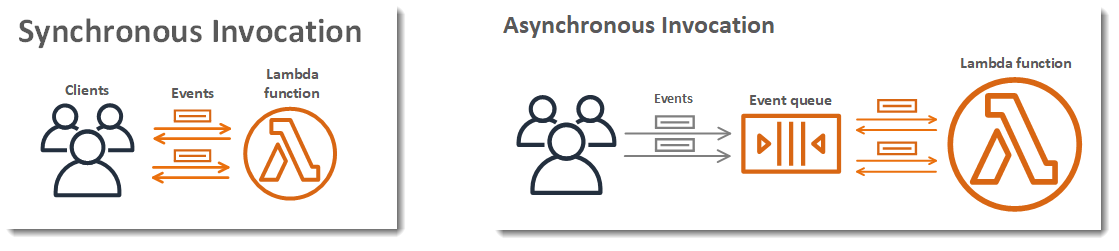
\includegraphics[scale=0.5]{Pictures/3_lambda.png}
    \caption{Lambda invocation types.}
    \label{fig:3_lambda_invocation}
\end{figure}

Synchronous invocation, where the caller waits for the function to process the event and return a
response, is commonly used in scenarios like API executions through Amazon API Gateway. Asynchronous
invocation is employed when the order of execution is not critical. In this case, events are placed
in a queue before being sent to the function, and AWS Lambda manages the function's invocation rate.
For asynchronous execution, AWS also provides services like Amazon Simple Queue Service (SQS) for
queueing messages or Amazon Simple Notification Service (SNS) for delivering messages to subscribing
endpoints or functions. These services can be directly integrated with Lambda to handle
event-driven, scalable computing architectures, allowing developers to focus on code rather than
infrastructure management.

\subsection{AWS RDS}
Amazon Relational Database Service (Amazon RDS) is a web service from AWS that simplifies setting
up, using, and scaling relational databases in the cloud. It offers scalable, cost-effective
solutions for standard industry relational databases, managing common administrative tasks, thus
allowing users to focus more on their applications and user engagement. As a fully managed service,
Amazon RDS handles the majority of management tasks, relieving users from manual and time-consuming
database maintenance. It supports various popular database engines, such as Amazon Aurora, MySQL,
MariaDB, PostgreSQL, Oracle, and SQL Server. Additionally, Amazon RDS provides deployment
flexibility, including on-premises options with Amazon RDS on AWS Outposts. This combination of
versatile database engine support, automated management, and deployment options make Amazon RDS a
comprehensive and user-friendly solution for managing relational databases in the AWS
Cloud\textsuperscript{\cite{tech_4}}.

\subsubsection{RDS vs DynamoDB}
AWS does not offer only SQL options with RDS; there is also DynamoDB, a NoSQL alternative for
different database needs. While RDS excels in structured data management and complex querying
capabilities via SQL, DynamoDB provides a flexible schema with key-value and document data models,
delivering quick and predictable performance. RDS is preferable for traditional applications that
need transactional support, complex joins, and other SQL operations. In contrast, DynamoDB is
tailored for modern applications that demand scalability, low-latency data access, and where
database management overhead should be minimized. The choice between RDS and DynamoDB hinges on the
application's data requirements and scalability demands.

\subsection{AWS SQS}
Amazon Simple Queue Service (SQS) is a fully managed message queuing service for microservices,
distributed systems, and serverless applications, offering secure and reliable data transfer without
losing messages or depending on other services' availability. Amazon SQS provides key benefits such
as security, with user-controlled access and server-side encryption options using AWS Key Management
Service, and durability, ensuring message storage across multiple servers. Its high availability is
maintained through a redundant infrastructure for consistent message access. The service is highly
scalable, processing each request independently to manage load spikes, and guarantees reliability by
locking messages during processing to support multiple producers and consumers. Amazon SQS also
allows for customization, like setting default delays on queues or storing large message contents on
Amazon S3 or DynamoDB. These features make Amazon SQS an efficient and versatile tool for handling
large volumes of messages in various application architectures, offering a combination of
reliability, scalability, security, and customization\textsuperscript{\cite{tech_5}}.

\subsection{AWS SNS}
Amazon Simple Notification Service (Amazon SNS) is a fully managed service offering effective
Pub/Sub messaging for both application-to-application (A2A) and application-to-person (A2P)
communication. It facilitates high-throughput, push-based messaging among distributed systems,
microservices, and serverless applications, integrating seamlessly with Amazon SQS, AWS Lambda, and
other services. A2P messaging extends capabilities to customer communications through SMS, push
notifications, and emails. Amazon SNS stands out for simplifying messaging architectures while
reducing costs through features like message filtering, batching, ordering, and deduplication. It
also enhances message durability with storage, delivery retries, and dead-letter queues.
Additionally, it supports strict FIFO message delivery, ensuring accuracy and consistency across
applications. This combination of features makes Amazon SNS a versatile tool for a wide range of
messaging scenarios, from system integration to direct customer
engagement\textsuperscript{\cite{tech_6}}.

\subsection{AWS Cognito}
Amazon Cognito is a comprehensive service designed to implement secure, frictionless customer
identity and access management (CIAM) in a scalable manner. With Amazon Cognito, you can offer a
smooth management of customer identity and access, thanks to its affordable and customizable
platform. It includes features such as adaptive authentication, support for compliance, and data
residency requirements.Amazon Cognito is capable of scaling to millions of users with a fully
managed, high-performance, and reliable identity store. It also provides access to federation using
OpenID Connect (OIDC) or SAML 2.0 and integrates with a broad range of AWS services and products.
This platform supports up to 50,000 active users per month for free under the AWS free tier plan,
making it a cost-effective solution for businesses of varying sizes\textsuperscript{\cite{tech_7}}.

\section{Firebase Cloud Messaging}
Firebase Cloud Messaging (FCM)\textsuperscript{\cite{tech_9}} is a powerful cloud solution for
messages on iOS, Android, and web applications for free. It provides a reliable and efficient
connection between servers and devices that allows for the delivery of notifications or messages.
FCM offers versatile messaging options including topic messaging, which allows you to send a message
to multiple devices that have opted in to a particular topic, device group messaging, allowing for
messages to devices that belong to a group, and direct messaging to individual devices. This
scalability makes it an essential tool for developers looking to engage their user base effectively,
with the added benefits of analytics and performance tracking.

\subsection{How it works}
Firebase Cloud Messaging employs a client-server architecture where the FCM backend is responsible
for handling and routing messages. The client app on a user's device communicates with the FCM via
an SDK, which manages the registration process and token generation. This token uniquely identifies
the app instance and enables secure message delivery to the device. Messages sent from the
developer's server to the FCM backend can be payload-specific, directing the FCM to deliver them as
notification or data messages. FCM then optimizes message delivery by queuing them, managing
priority, and even aggregating messages for network efficiency. This architecture supports a high
level of scalability and reliability in delivering messages across platforms and devices globally.

\begin{figure}
    \centering
    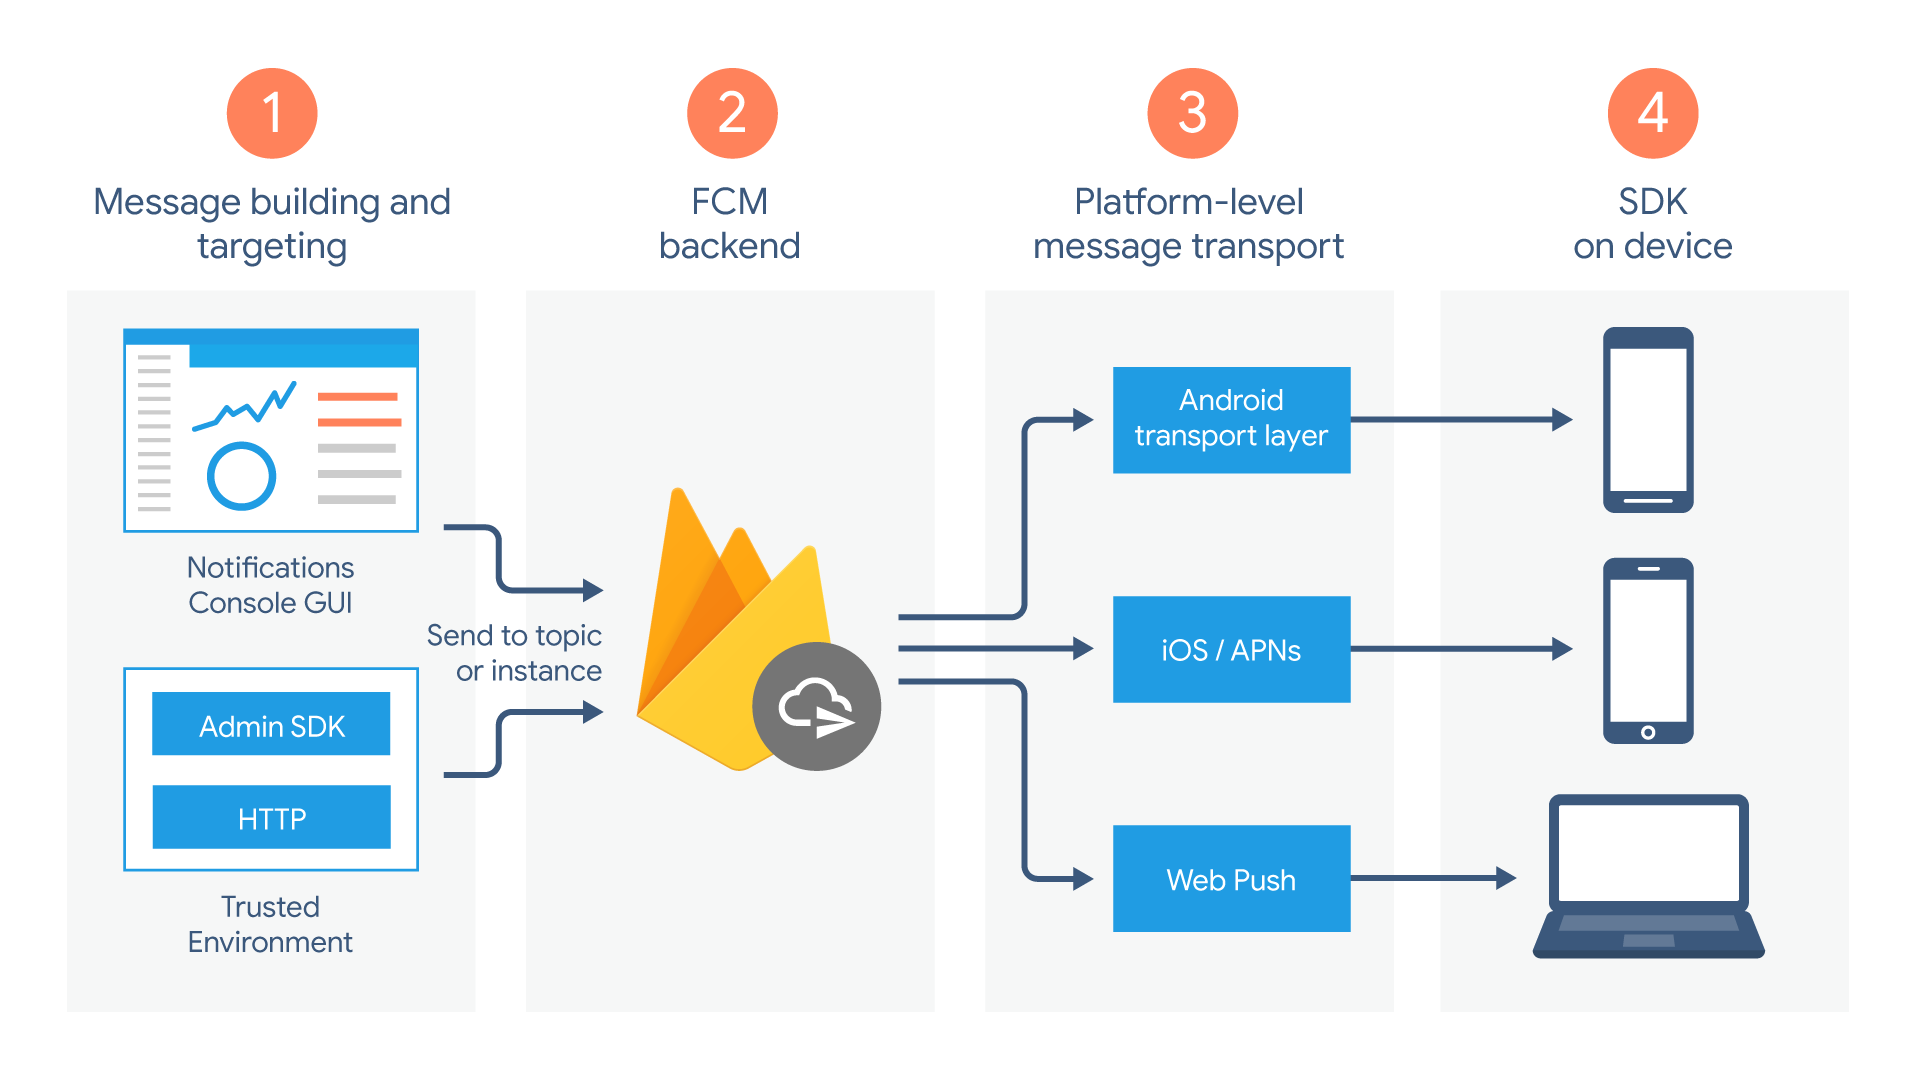
\includegraphics[scale=0.2]{Pictures/3_firebase.png}
    \caption{FCM architecture.}
    \label{fig:3_firebase}
\end{figure}

The image \ref{fig:3_firebase} show the FCM's operational architecture:

\begin{enumerate}
    \item Tools for crafting message requests, including a GUI via the Notifications composer for
          notifications, and server environments like Cloud Functions for Firebase or App Engine,
          supported by the Firebase Admin SDK or FCM server protocol, for comprehensive message type
          handling.
    \item The central FCM server that handles incoming message requests, manages topic-based message
          distribution, and assigns metadata like message IDs.
    \item A device-level transport system that ensures messages reach their destination, varying by
          platform: Android devices, Apple devices and Web push protocols for browsers
    \item The FCM SDK, which resides on the end-user's device, and is responsible for displaying
          notifications or processing messages, depending on the app's state and custom logic.
\end{enumerate}

\section{GO Language}
For my project, I chose the Go language\textsuperscript{\cite{tech_10}} due to its inherent
cloud-native characteristics and enhanced performance in cloud environments. It presents numerous
advantages and capabilities:

\begin{itemize}
    \item Concurrency in Cloud Computing: Go is tailored for building highly reliable concurrent
          applications, a necessity in cloud computing where coordinating access to shared resources is
          crucial. This makes Go an excellent choice for scalable cloud systems.
    \item Development Cycle and Server Performance: Go addresses the trade-off between development
          cycle time and server performance. A significant portion of Cloud Native Computing Foundation
          projects use Go. Its fast build times, lower memory and CPU utilization, and instant server
          start-up times make it a cost-effective option for cloud applications.
    \item Addressing Modern Cloud Challenges: Go provides standard idiomatic APIs and built-in
          concurrency to leverage multicore processors. Its low-latency and "no knob" tuning offer a
          balance between performance and productivity, enabling teams to adapt quickly to changing needs.
    \item Strong Ecosystem for Service Development: Go's standard library includes tools for HTTP
          servers and clients, JSON/XML parsing, SQL databases, and security/encryption. The runtime
          includes tools for race detection, benchmarking, code generation, and static code analysis.
          Major cloud providers and open-source libraries offer Go APIs, supporting a wide range of
          services and functionalities.
\end{itemize}

It have the drawback too, it has faced criticism for its until-recent lack of generics, leading to
less flexible code, and its verbose error handling approach. While Go's standard library is
comprehensive, it sometimes falls short in specialized third-party libraries compared to other
languages. In essence, Go excels in backend and cloud services development but might not be ideal
for all project types.

\subsection{GO CDK}
The Go Cloud Development Kit\textsuperscript{\cite{tech_11}} is an open-source project aimed at
enhancing the experience of developing cloud applications with Go. It provides vendor-neutral,
commonly used generic APIs that work across different cloud providers, supporting hybrid cloud
deployments and the integration of on-premises (local) and cloud tools. Go CDK's main focus is on
portable APIs for cloud programming, targeting major cloud providers like AWS, GCP, and Azure, along
with local (on-prem) implementations. The project enables developers to write application code once
using these APIs, test locally, and then deploy to a cloud provider with minimal changes. The Go CDK
is open-source and released under the Apache 2.0 License. \newline\newline
The Go CDK provides APIs like blob.Bucket or runtimevar.Variable as specific, concrete types rather
than interfaces. This design distinguishes the generic logic from the specific interface. The
generic logic resides in what we call the 'portable type,' whereas the 'driver' represents the
interface. This is illustrated in figure \ref{fig:3_go_cdk}.

\begin{figure}
    \centering
    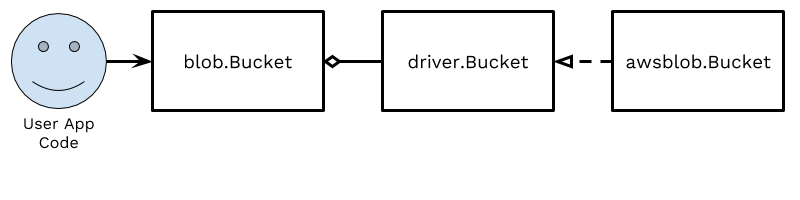
\includegraphics[scale=0.5]{Pictures/3_go_cdk.png}
    \caption{Go CDK API architecture.}
    \label{fig:3_go_cdk}
\end{figure}

This approach offers several advantages:
\begin{itemize}
    \item The portable type can handle complex logic internally, simplifying the driver's interface.
          For example, in the blob service, the NewWriter method of the portable type can determine the
          content type before interacting with the driver.
    \item It allows for the addition of new methods to the portable type without affecting backward
          compatibility, unlike modifying an interface which would be a breaking change.
    \item The portable type can seamlessly integrate new operations introduced in the driver through
          optional interfaces, eliminating the need for the user to perform type assertions.
\end{itemize}

\subsection{GORM}
GORM\textsuperscript{\cite{tech_12}} is a prominent ORM (Object-Relational Mapping) library for Go
(Golang), designed to be developer-friendly. It offers a full-featured ORM system with capabilities
such as associations (various relationship types), hooks (for create, save, update, delete, find
operations), and eager loading using Preload and Joins. GORM supports transactions, nested
transactions, context, prepared statement mode, and dry-run mode. It also provides functionality for
batch insert, SQL building, upserts, locking, and auto migrations. The library includes a logger,
extendable plugins, and is test-backed for each feature. Additionally, GORM supports composite
primary keys, indexes, and constraints, emphasizing its flexibility and developer-friendly nature.

\section{Serverless framework}
The Serverless Framework\textsuperscript{\cite{tech_13}} is a leading tool for deploying serverless
architectures. Developed after the release of AWS Lambda in 2014, it enables building applications
on cloud infrastructure that auto-scales and incurs no charges when idle. Key highlights include:

\begin{itemize}
    \item Empowering developers to focus more on building and less on managing.
    \item Supporting a wide range of serverless use-cases.
    \item Automated deployment of both code and infrastructure.
    \item Simple syntax for deploying AWS Lambda functions without needing in-depth cloud expertise.
    \item Multi-language support.
    \item Full lifecycle management of serverless architecture.
    \item Built-in support for multiple stages and environments.
    \item Extensibility through plugins.
\end{itemize}

The Framework streamlines serverless application development, offering tools for building,
deploying, updating, monitoring, and troubleshooting serverless architectures.

\subsection{Pros and cons}
The Serverless Framework offers a host of benefits for serverless architecture, such as facilitating
more efficient building with less management, supporting a wide range of use-cases, automating code
and infrastructure deployment, and providing simple syntax for safe AWS Lambda function deployment.
It supports multiple languages and manages the full lifecycle of serverless architecture,
accommodating large projects and teams with multi-domain and multi-environment support. The
framework is also highly extensible through its plugin ecosystem. However, it presents challenges
like a steep learning curve for newcomers, potential dependency issues, limited control over fine
infrastructure details, complexities in handling large-scale projects, and possible performance
bottlenecks. Also the variability in plugin reliability, the risk of vendor lock-in, and
challenges in cost management are significant considerations.

\subsection{Alternatives}

\begin{figure}
    \centering
    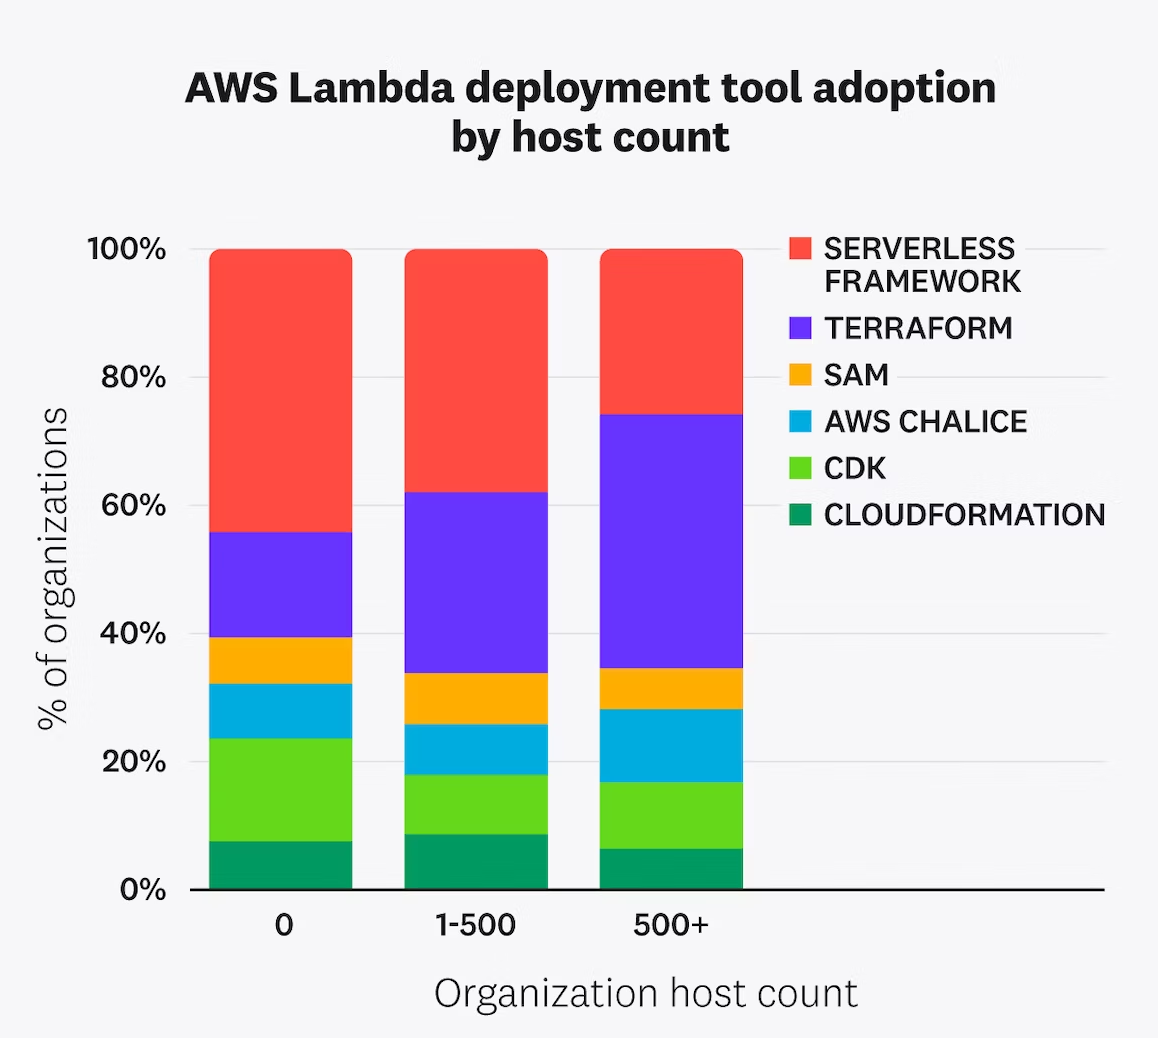
\includegraphics[scale=0.5]{Pictures/3_serverless_framework.png}
    \caption{Serverless Framework alternatives.}
    \label{fig:3_serverless_alternatives}
\end{figure}

Based on the image \ref{fig:3_serverless_alternatives} taken from a Datadog
research\textsuperscript{\cite{tech_14}}, it is evident that there are several alternatives to the
Serverless Framework for deploying functions, and their adoption varies according to the size of the
organization, measured by host count. In smaller companies with zero hosts, the Serverless Framework
is the clear frontrunner, indicating its preference among startups or for small-scale projects. For
mid-sized organizations, with host counts between 1 and 500, there is a more even split between the
Serverless Framework and Terraform, showing that both tools are well-suited for medium-scale
operations. However, in larger companies with over 500 hosts, Terraform emerges as the dominant
tool. This trend suggests that Terraform's versatility, its support for multiple cloud providers,
and its widespread adoption by DevOps teams make it the preferred choice for larger organizations
that likely have more complex and diverse cloud infrastructures.

\section{Flutter}
Flutter\textsuperscript{\cite{tech_15}} is an open-source UI software development kit created by
Google. It's used for building natively compiled applications for mobile, web, and desktop from a
single codebase. Flutter provides a fast development cycle with a "hot reload" feature that allows
instant updates without losing the state of the app. It offers expressive and flexible UI with a
rich set of widgets and a layered architecture that enables full customization. Flutter's native
performance is achieved through the use of Dart, which compiles to ARM or JavaScript code. This
toolkit is popular for its ability to create visually attractive and natively compiled applications
across platforms efficiently.

\subsection{Pros and cons}
Flutter, as a framework for app development, offers several compelling advantages alongside a few
drawbacks. Its ability to maintain consistency across multiple platforms with a single codebase
streamlines development, while the stateful hot reload feature significantly boosts developer
productivity. The framework's growing popularity is evident from its strong community support and
open-source nature, which fosters continual improvement and innovation. Flutter's approach to app
development with customizable widgets and excellent documentation facilitates faster and more
flexible app creation. However, being a relatively new entrant in the cross-platform arena, it faces
challenges such as limited learning resources, fewer plugins and packages compared to more
established frameworks, and larger app sizes due to its use of built-in widgets. Additionally, Dart,
the programming language for Flutter, has a smaller community, which might limit resources for
learning and development. These factors make Flutter a powerful but nuanced choice for app
developers, balancing its efficiency and ease of use against the considerations of newness and
community size.

\subsection{Architecture}
As depicted in figure \ref{fig:3_flutter_architecture}, Flutter is constructed as a modular, layered
framework. It comprises a set of autonomous libraries where each is built upon the layer beneath it.
There's no special access granted to any layer over the one it rests on, ensuring a democratic
structure. Additionally, the framework is engineered to be adaptable, with each segment crafted to
be optional and replaceable.

\begin{figure}
    \centering
    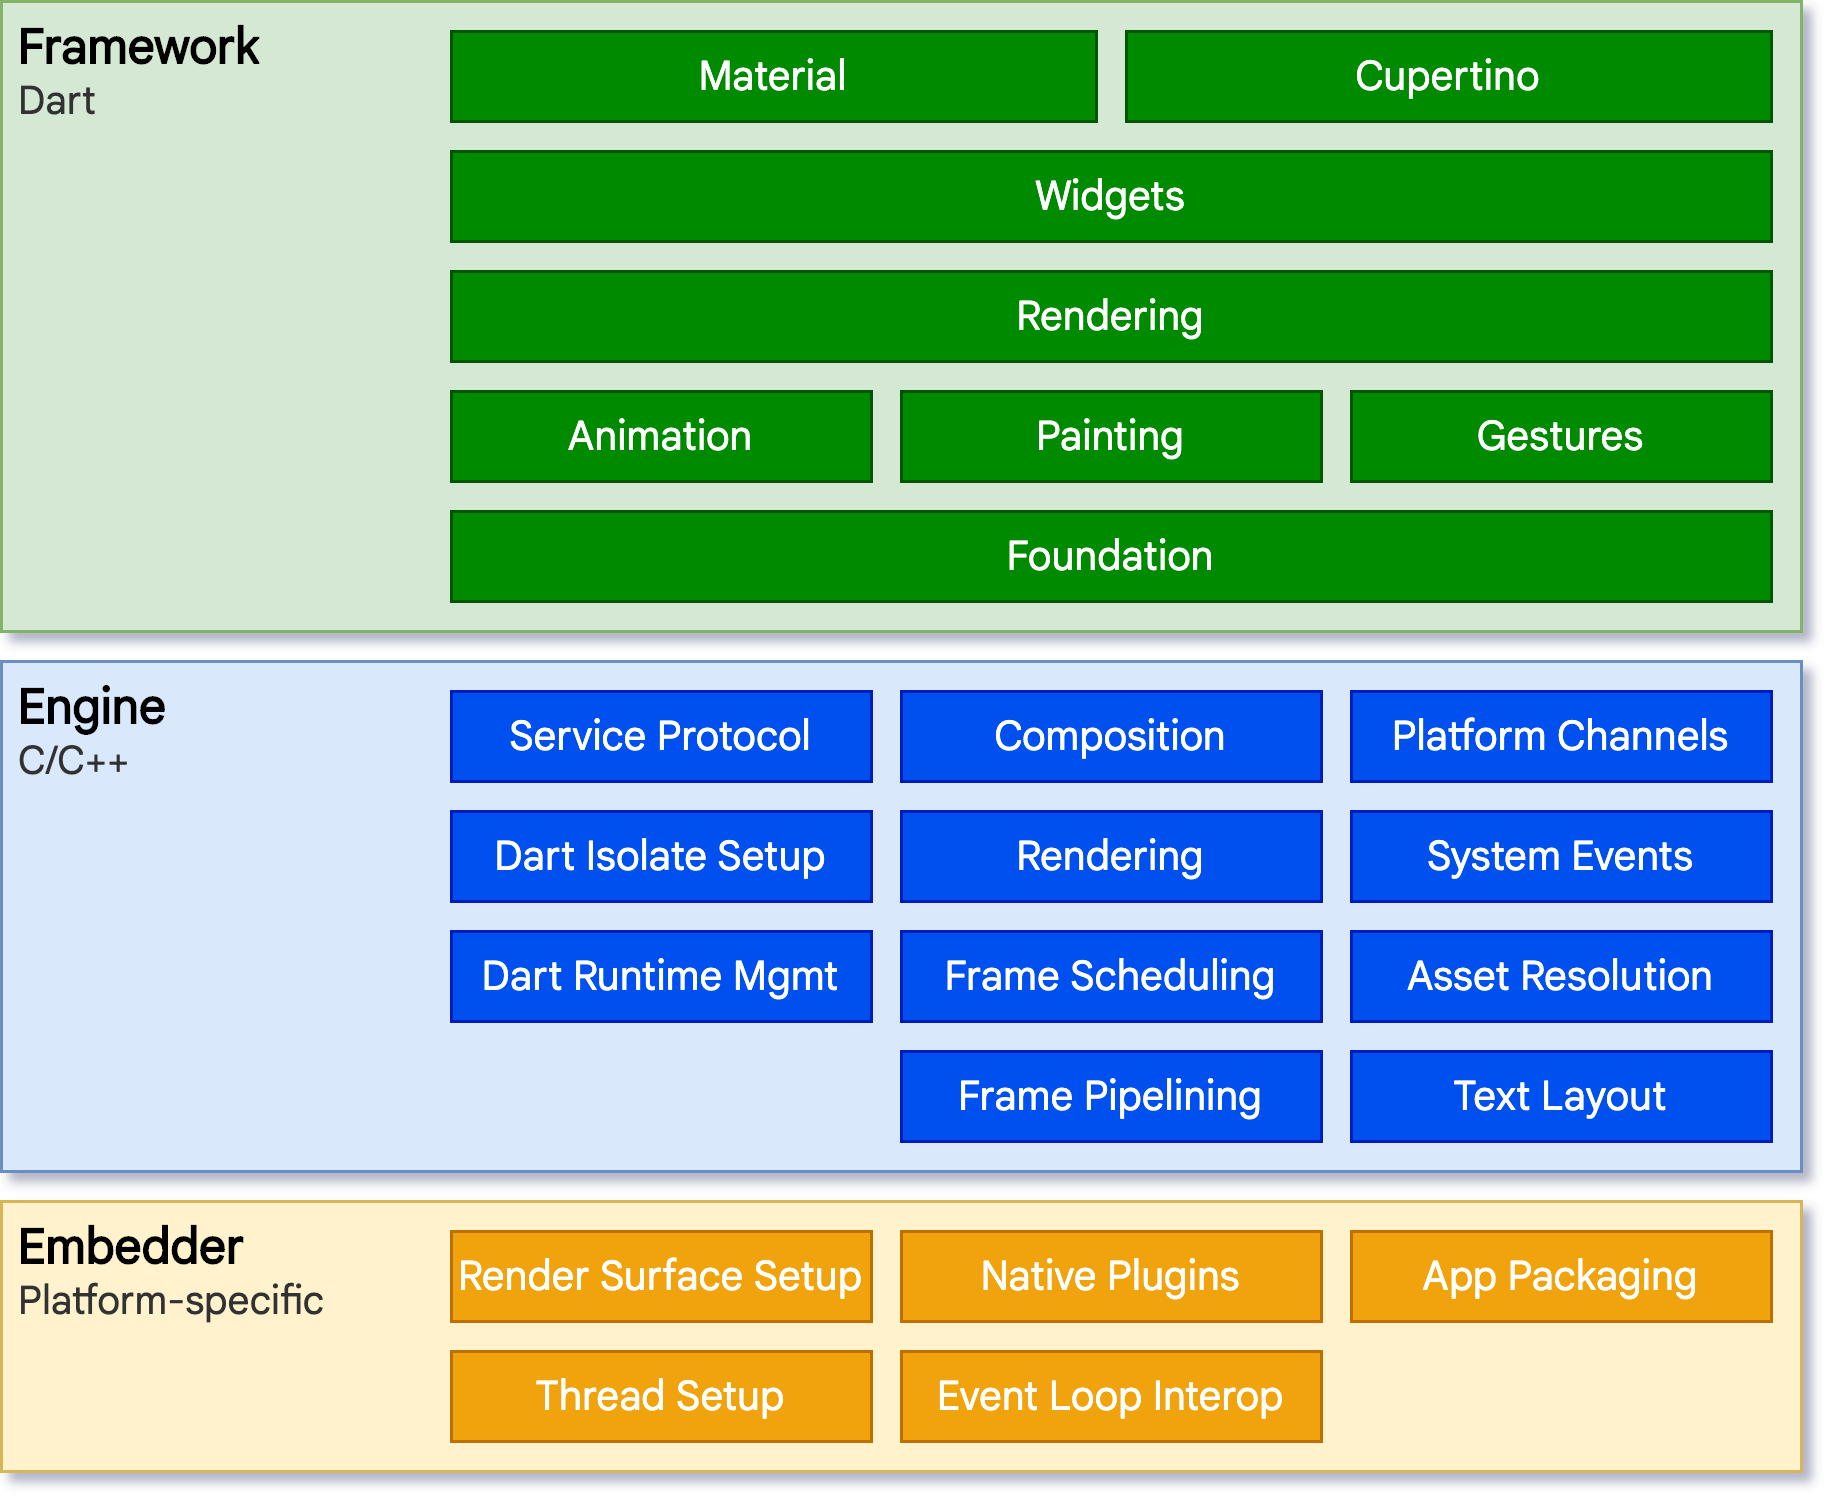
\includegraphics[scale=0.2]{Pictures/3_flutter.png}
    \caption{Flutter architecture.}
    \label{fig:3_flutter_architecture}
\end{figure}

To the base operating system, Flutter apps are wrapped and delivered just like any native app. The
platform-specific embedder acts as the initial entry point, interfacing with the OS for critical
services such as rendering surfaces, accessibility, inputs, and managing the messaging event loop.
This embedder layer is adaptable, written in the native languages of the platform such as Java and
C++ for Android, Objective-C/Objective-C++ for iOS and macOS, C++ for Windows and Linux, and
JavaScript for the web. Flutter's flexibility allows its code to be embedded within existing apps as
a module, or to form the entirety of a new application, supported by a variety of embedders tailored
for common target platforms, as well as third-party options.
\newline\newline
Central to Flutter's functionality is the engine layer, primarily crafted in C++. This engine
underpins every Flutter app by providing the essential components they require. It's tasked with
rasterizing composited scenes for painting new frames and underlies the core API of Flutter,
encompassing graphics (employing Impeller on iOS, soon on Android, and Skia elsewhere), text, file
and network I/O, accessibility, plugin infrastructure, and the Dart runtime with compilation tools.
\newline\newline
The bridge between the Flutter engine and the framework is dart:ui, which translates the engine's
C++ capabilities into Dart classes. This critical library introduces base primitives, enabling the
manipulation of input, graphics, and text rendering. Although the core Flutter framework is compact,
it is extendable, with numerous high-level functions available through additional packages, not
unlike the independent libraries stacked in the image, which collectively form the robust and
extensible framework that Flutter is known for.

\subsection{Alternatives}
Two major alternatives to Flutter for app development are React Native and Angular.
\newline\newline
React Native\textsuperscript{\cite{tech_16}}, developed by Facebook, is an open-source framework
tailored for building mobile applications. It allows developers to create natively rendered apps for
both iOS and Android using React, a popular JavaScript library. This framework embraces a 'learn
once, write anywhere' philosophy, enabling the use of a single codebase for multiple platforms while
retaining the capability to include platform-specific features. Known for its time and resource
efficiency, React Native can seamlessly integrate with existing native code, offering versatility in
development. It features live reloading for immediate reflection of code changes, boosting developer
productivity. With extensive community support, a wealth of libraries, and third-party plugin
compatibility, React Native is ideal for developers aiming for efficient cross-platform development
with a strong native performance and feel.
\newline\newline
Angular\textsuperscript{\cite{tech_17}}, developed by Google, is a comprehensive solution for web
application development. This platform and framework are geared towards building single-page client
applications using HTML and TypeScript. Angular streamlines the development and testing process with
tools for declarative templates, dependency injection, and integrated best practices. It features a
two-way data binding, reducing the need for additional code and enhancing efficiency for interactive
applications. Angular's architecture supports the rapid development of readable, maintainable, and
testable code, making it suitable for enterprise-level and complex web projects that demand
scalability and productivity. With its extensive libraries and strong community support, Angular is
an excellent choice for creating dynamic, high-performance web applications.

\chapter{Kube Platform}
In this chapter, we commence on an in-depth exploration of the Kube platform, an implementation of
innovative ERP platform prototype. We start by outlining the fundamental requirements that have
shaped the development of the Kube platform, highlighting the strategic objectives, technical needs,
and business logic that inform its design. This leads us into a detailed examination of the
platform’s final architecture, which showcases a Microservices framework implemented through a
Function as a Service (FaaS) model, using AWS services. We then transition to practical
applications, where specific use cases demonstrate the platform's operational flow and its
real-world applicability. The chapter ends with a focus on the client application, delving into the
design and development of a user interface using Flutter, which not only complements the platform's
robust backend but also enhances the overall user experience. Throughout this chapter, we aim to
unravel the complexities of the Kube platform, illustrating its role as a transformative force in
the field of enterprise resource planning and highlighting its potential.

\section{Requirements}
Before starting development, requirements are established to define the properties of the product.
It's important that these requirements are thorough and coherent, covering all necessary features
without conflicts or inconsistencies. However, creating these documents can be challenging and
errors may occur, such as incomplete or ambiguous feature descriptions, redundancy, or important
details being omitted. To address these challenges, software engineering techniques have been
developed to formalize the requirements and minimize the occurrence of errors.
\newline\newline
ISO/IEC 25010\textsuperscript{\cite{ch5_1}}, an international standard, serves as a comprehensive
framework for assessing software product quality. This standard enumerates several key quality
characteristics, including functionality, reliability, usability, efficiency, maintainability,
security, compatibility, and portability. Its widespread application in software engineering and
quality assurance offers a standardized approach to evaluating and articulating software quality.
This facilitates more informed decisions in software acquisition, development, and maintenance.
ISO/IEC 25010 aids in identifying the actors involved and delineating both functional and
non-functional requirements.

\subsection{Stakeholders}
A stakeholder refers to any role, person, group, or organization that has an interest in a software
project or system being developed. This could include end-users, customers, investors, project
managers, developers and other individuals or groups involved in the development, deployment, and
maintenance of the software. Identifying all relevant stakeholders is important for considering
diverse perspectives and generating relevant requirements for the system. As shown in Table
\ref{tab:5_stakeholders}, numerous stakeholders play a role in the process.

\begin{table}[h]
    \centering
    \begin{tabular}{|l|p{10cm}|}
        \hline
        \textbf{Stakeholder} & \textbf{Description}                                                                                                                                                 \\ \hline
        End-users            & These are the people who will use the ERP system in their day-to-day work. They may include employees from various departments within the organization.              \\ \hline
        Developers           & These are the individuals responsible for creating the software code that makes up the ERP system.                                                                   \\ \hline
        Admin/IT staff       & These are the individuals responsible for installing, configuring, and maintaining the ERP system.                                                                   \\ \hline
        Customers            & These are the organizations or businesses that are purchasing the ERP system. They have a vested interest in ensuring the system meets their needs and requirements. \\ \hline
        Vendors              & These are the organizations that provide the ERP software and related services, such as installation, configuration, and support.                                    \\ \hline
        Cloud Vendors        & These hosts the system and provide the necessary infrastructure for its operation. They are responsible for system availability, scalability, and security.          \\ \hline
    \end{tabular}
    \caption{Stakeholders of a Cloud ERP System.}
    \label{tab:5_stakeholders}
\end{table}

\subsection{Functional and Non-functional}
Functional requirements and non-functional requirements are two types of requirements that are used
to specify what a system or software application should do and how it should perform. They are
important for the successful development and implementation of a system or software application. The
functional requirements ensure that the software application meets the needs of its users, while the
non-functional requirements ensure that the system is reliable, efficient, and secure.

\subsubsection{Functional requirements}
Functional requirements describe what the system should do in terms of its functionalities,
features, and capabilities. They define the specific tasks that the software application should be
able to perform to meet the needs of its users. For distinguish one requirement from another it is
important to assign for each functionality an ID, in order to easy identify it and trace throughout
the life cycle of the project (Table \ref{tab:functional_requirements}).

\begin{table}
    \centering
    \begin{tabular}{|l|p{10cm}|}
        \hline
        ID     & Description                                           \\ \hline
        FR1    & Sign-up users by email and password                   \\ \hline
        FR2    & Login users by email and password                     \\ \hline
        FR3    & Logout users                                          \\ \hline
        FR4    & Activate notifications                                \\ \hline
        FR5    & Deactivate notifications                              \\ \hline
        FR6    & View chart for andamento mensile degli ordini         \\ \hline
        FR7    & View chart for distribuzione degli ordini per cliente \\ \hline
        FR8    & Customize the menu bar                                \\ \hline
        FR9    & View the log of the platform events                   \\ \hline
        FR9.1  & View the detailed log of an event                     \\ \hline
        FR9.2  & Delete a log event                                    \\ \hline
        FR10   & View the customers list                               \\ \hline
        FR10.1 & View the detailed customer                            \\ \hline
        FR10.2 & Insert a customer                                     \\ \hline
        FR10.3 & Update a customer                                     \\ \hline
        FR10.4 & Delete a customer                                     \\ \hline
        FR11   & View the sales order list                             \\ \hline
        FR11.1 & View the detailed sales order with sales lines        \\ \hline
        FR11.2 & Insert a sales order                                  \\ \hline
        FR11.3 & Update a sales order                                  \\ \hline
        FR11.4 & Delete a sales order                                  \\ \hline
        FR11.5 & Insert a sales order line                             \\ \hline
        FR11.6 & Update a sales order line                             \\ \hline
        FR11.7 & Delete a sales order line                             \\ \hline
        FR12   & Launch the posting order event                        \\ \hline
        FR13   & show notifications of change status on order          \\ \hline
        FR14   & View the shipment list                                \\ \hline
        FR14.1 & View the detailed shipment with sales lines           \\ \hline
        FR14.2 & Delete a shipment                                     \\ \hline
        FR15   & View the invoice list                                 \\ \hline
        FR15.1 & View the detailed invoice with sales lines            \\ \hline
        FR15.2 & Delete an invoice                                     \\ \hline
    \end{tabular}
    \caption{Functional requirements for the platform.}
    \label{tab:functional_requirements}
\end{table}

\subsubsection{Non-functional requirements}
Non-functional requirements describe how the system should perform in terms of its functionality,
reliability, usability, efficiency, maintainability, security, compatibility, and portability, all
aspects that are not directly related to the specific functionalities to be implemented. They refer
to operating methods and constraints, such as response times, supported platforms, choice of
languages, required resources, tools and various implementation techniques. They must be measurable
and may be more critical than functional requirements. They are identified with a unique code and it
is also necessary to specify their type associated to the ISO properties and which functional
requirements they refer to (Table \ref{tab:non_functional_requirements}).

\begin{table}
    \centering
    \begin{tabular}{|l|c|p{9cm}|}
        \hline
        ID   & Type            & Description                                                        \\ \hline
        NFR1 & Usabilty        & Application should be used with no training by any user            \\ \hline
        NFR2 & Efficiency      & All functions should complete in < 0.5 sec                         \\ \hline
        NFR2 & Efficiency      & All functions must optimize the resource utilization               \\ \hline
        NFR3 & Portability     & System must work on Chrome, Firefox, Safari, Edge, Android and iOS \\ \hline
        NFR4 & Portability     & No installation is needed                                          \\ \hline
        NFR5 & Compatibility   & Platform must be compatible with Azure and AWS cloud               \\ \hline
        NFR6 & Security        & All data must be stored in a secure database                       \\ \hline
        NFR7 & Maintainability & All functionalities must be tested indipendently                   \\ \hline
        NFR8 & Reliabilty      & Downtime allowed is of one hour per year                           \\ \hline
    \end{tabular}
    \caption{Non-functional requirements for the platform.}
    \label{tab:non_functional_requirements}
\end{table}

\section{Server application}
In this section, we will discuss the final architecture designed for the Kube platform, encompassing
its data structures and services. We will explore the database setup, highlighting the tables
crafted for each microservice. Following this, we'll shed light on the REST APIs tailored for every
microservice, along with the integration of queues and events designed for asynchronous event
management. Concluding our discussion, we'll outline a SAGA implementation that has been
incorporated into the platform.
\newpage

\subsection{Final Architecture}
% TODO Aumenta i font e metti le frecce su events
\begin{figure}
    \centering
    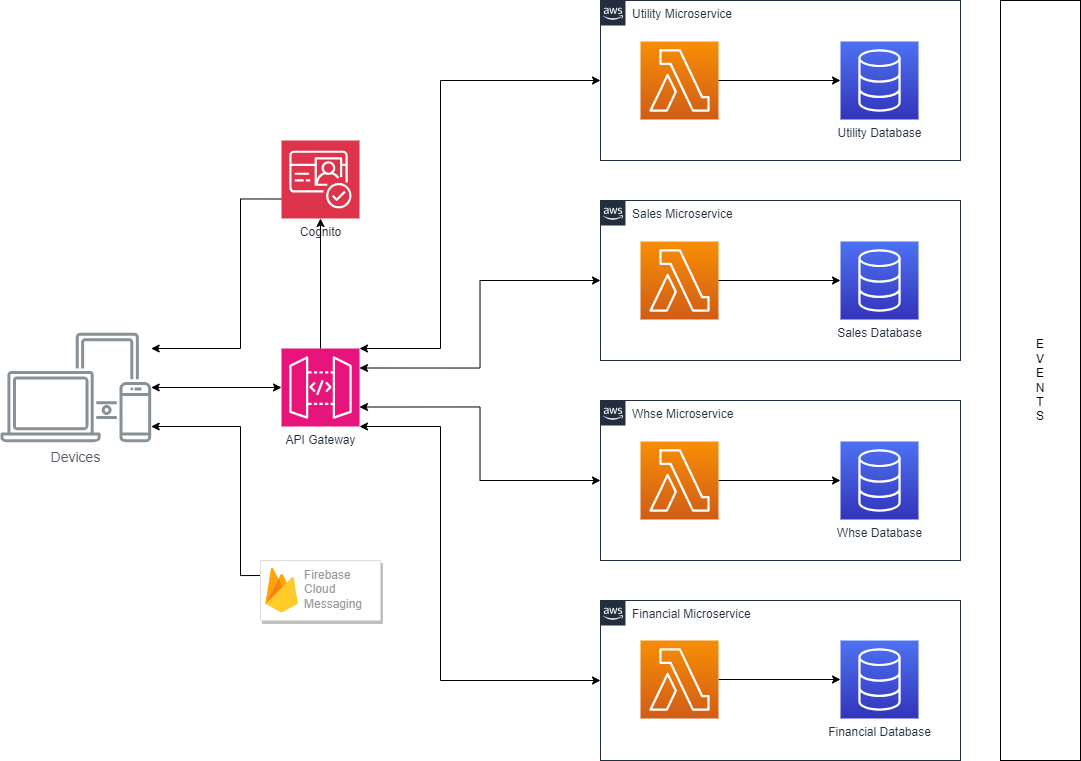
\includegraphics[scale=0.35]{Pictures/5_architecture.png}
    \caption{Final architecture of the platform.}
    \label{fig:5_architecture}
\end{figure}
The architecture diagram in Figure \ref{fig:5_architecture} showcases a modern, serverless
microservices-based architecture for the Kube system. Here's a description based on the elements and
their interconnections:

\begin{itemize}
    \item \textbf{User Authentication}: the service which is responsible for user authentication is
          'Cognito'. It is the entry point for security, ensuring that only authenticated users can
          interact with the platform and with all the API.

    \item \textbf{Firebase Cloud Messaging}: At the bottom of the diagram, we can see 'Firebase Cloud Messaging',
          it is an integration with a cloud solution for sending notifications to devices, allowing for
          real-time user engagement.

    \item \textbf{API Gateway}: The 'API Gateway' is the central hub through which all client
          requests pass. It acts as a front door, directing incoming requests from various devices (such as
          computers and mobile phones) to the appropriate microservices.

    \item \textbf{Microservices Architecture}: Actually each microservice is deployed to AWS (Amazon
          Web Services), and utilize various AWS serverless features for optimizing performance.

          \begin{itemize}
              \item \textbf{Utility Microservice}: This service handles log functions and events,
                    and is backed by a 'Utility Database' for storing log records. It also manage
                    home page graph function and data and navigations/menu API and data.
              \item \textbf{Sales Microservice}: Dedicated to handling sales-related operations,
                    like handle customer and sales order, this service interacts with a 'Sales
                    Database'.
              \item \textbf{Whse Microservice}: this service manages shipment and warehouse-related
                    data, backed by its own 'Whse Database'.
              \item \textbf{Financial Microservice}: This handles financial transactions and invoice, with a
                    separate 'Financial Database' for storing related records.
          \end{itemize}

    \item \textbf{Database Pattern}: The architecture uses a database-per-microservice pattern with SQL
          databases, ensuring that each service has its own datastore, thus maintaining database isolation and
          decoupling services.

    \item \textbf{Event-Driven Architecture}: all microservices are connected through an
          event-driven architecture, which allows them to communicate asynchronously and facilitates
          loose coupling. This architecture is implemented using Amazon Simple Queue Service (SQS)
          and Amazon Simple Notification Service (SNS), which are managed message queues and
          notification services.
\end{itemize}

All services are managed and deployed using the serverless framework, which allows to easily
integrate a CI/CD pipeline manage the entire infrastructure as code. With this setup, the platform
can be easily deployed to other cloud providers and add other cloud services and features. How we
can see, the Kube platform's architecture is designed to be scalable, flexible, and maintainable,
with a focus on modern cloud-native principles and best practices for microservices development.

\subsubsection{Microservices components}
\begin{figure}
    \centering
    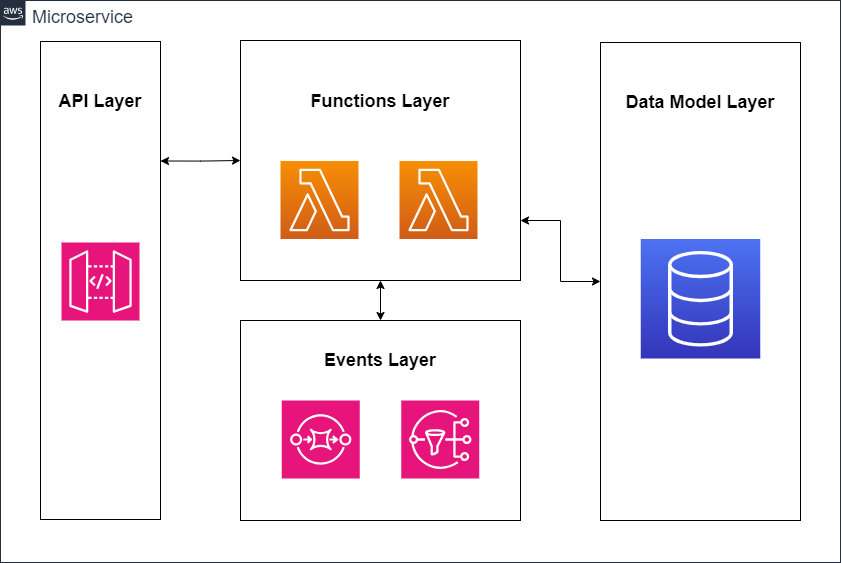
\includegraphics[scale=0.28]{Pictures/5_microservizio.png}
    \caption{Microservices components.}
    \label{fig:5_microservices}
\end{figure}

Each microservice in the Kube platform is a composite of four essential components that work in
concert to deliver its specific functionality:

\begin{table}
    \centering
    \begin{tabular}{|c|c|m{8.5cm}|}
        \hline
        \textbf{Component}   & \textbf{Service} & \textbf{Description}                                                                                                                                                                                                                                                                                                                                                                                                \\ \hline
        \textbf{Data Models} & RDS              & At the core of each microservice is a set of data models. These models define the structure of the data that the microservice handles, ensuring data integrity and consistency. By having its own models, each microservice encapsulates the necessary information to perform its tasks, leading to a clear delineation of responsibilities within the system.                                                      \\ \hline
        \textbf{REST APIs}   & API Gateway      & The REST APIs serve as the interfaces through which external services or client applications interact with the microservices. These APIs are carefully designed to provide a clear and consistent contract for accessing and manipulating data. They follow REST principles, allowing for stateless communication and enabling clients to perform standard HTTP operations such as GET, POST, PATCH, and DELETE.    \\ \hline
        \textbf{Functions}   & Lambda           & The functions are the operational units within each microservice, containing the business logic that processes requests, manipulates data models, and performs the necessary computations. These functions are likely implemented as serverless functions, which are executed in response to events, scaling automatically with the number of requests and reducing the need for managing server infrastructure.    \\ \hline
        \textbf{Events}      & SNS, SQS         & Each microservice also incorporates an event-driven mechanism, signaling and reacting to various conditions and triggers. These events facilitate asynchronous communication between microservices, thereby enhancing the platform's responsiveness and efficiency. By decoupling microservices through events, the system can better handle load variations and failure modes, contributing to overall resilience. \\ \hline
    \end{tabular}
    \caption{Microservices components.}
    \label{tab:microservices_components}
\end{table}

Together, these components create a modular and cohesive microservice that is self-contained,
scalable, and robust. The data models ensure that each service can independently manage its segment
of the data. The REST APIs provide the necessary endpoints for interaction, while the functions
encapsulate the business logic. Finally, the event system allows the services to react to and
communicate changes across the platform without direct coupling, promoting a reactive architecture
that can quickly adapt to changing conditions.
% eventually consistent is enough because not critical data and not all system is coupled

\subsection{Code Structure}
In our microservices architecture, all lambda functions are written in the Go language. This
decision was influenced by several key factors. Firstly, Go is a compiled language, which leads to
significantly faster execution times and results in smaller executable files. Another important
reason for choosing Go is the availability of the Go CDK library. This library is unique to Go and
aids in making functions as portable as possible across different cloud providers. While it's true
that shifting functions between providers requires some manual adjustments, the process could be
streamlined by developing CLI tools for automation.
\newline\newline
However, adopting Go was not without its challenges. Unlike object-oriented languages, Go doesn't
fully integrate all object-oriented principles. It has its own way of handling certain programming
concepts, which required a learning curve. Additionally, Go is not as versatile in some aspects; for
instance, the main function is bound to have a dedicated 'main' package. This can pose difficulties
in managing multiple functions, each with its own 'main,' making the overall management a complex
task.

\begin{figure}
    \centering
    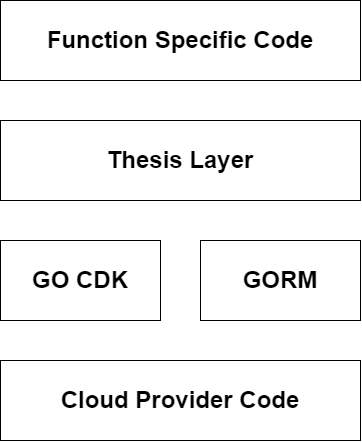
\includegraphics[scale=0.3]{Pictures/5_stack_framework.png}
    \caption{Stack abstractions layer.}
    \label{fig:5_stack_framework}
\end{figure}

In every function architecture, I've implemented an abstraction layer specifically designed for
managing REST APIs of various resources. This unified approach, applied across all microservices, is
facilitated by a layer we've named 'thesis.' Built on top of the GORM and Go CDK libraries, this
layer simplifies and accelerates API management. Connecting a GORM model to a 'thesis' layer
structure called 'page' requires minimal coding. The 'page' concept is central to our approach: it
automatically generates a suite of REST APIs for a resource, significantly reducing development time
and standardizing structures across resources. Moreover, these 'pages' can define a UI schema, which
clients can use to dynamically build pages for resources in their applications. The APIs that are
automatically constructed from a GORM model are structured as indicated inside the following tables.

\subsubsection{http://api.example.com/:pageid?field=value}
\begin{table}
    \centering
    \begin{tabular}{|m{2cm}|m{10cm}|}
        \hline
        \textbf{Method} & \textbf{Description}                                                                                                        \\ \hline
        \textbf{GET}    &
        Returns the list of records linked to the page. The records can be filtered by inserting the fields to be filtered in the URL's query string. \\ \hline
        \textbf{POST}   &
        Creates a new record in the table linked to the page.                                                                                         \\ \hline
        \textbf{PATCH}  &
        Edits the record in the table linked to the page.                                                                                             \\ \hline
        \textbf{DELETE} &
        Deletes records linked to the page. The records can be filtered by inserting the fields to be filtered in the URL's query string.             \\ \hline
    \end{tabular}
    \caption{REST API for page.}
    \label{tab:api_rest_1}
\end{table}

\subsubsection{http://api.example.com/:pageid/schema}
\begin{table}
    \centering
    \begin{tabular}{|m{2cm}|m{10cm}|}
        \hline
        \textbf{Method} & \textbf{Description}                     \\ \hline
        \textbf{GET}    &
        Returns the UI schema for building the page in the client. \\ \hline
        \textbf{POST}   &
        Not allowed.                                               \\ \hline
        \textbf{PATCH}  &
        Not allowed.                                               \\ \hline
        \textbf{DELETE} &
        Not allowed.                                               \\ \hline
    \end{tabular}
    \caption{Methods for page schema.}
    \label{tab:api_rest_2}
\end{table}

\subsubsection{http://api.example.com/:pageid/button?button\_id=value}
\begin{table}
    \centering
    \begin{tabular}{|m{2cm}|m{10cm}|}
        \hline
        \textbf{Method} & \textbf{Description}                                   \\ \hline
        \textbf{GET}    &
        Initiates the functionality linked to the button and returns the result. \\ \hline
        \textbf{POST}   &
        Not allowed.                                                             \\ \hline
        \textbf{PATCH}  &
        Not allowed.                                                             \\ \hline
        \textbf{DELETE} &
        Not allowed.                                                             \\ \hline
    \end{tabular}
    \caption{Methods for page buttons.}
    \label{tab:api_rest_3}
\end{table}

\subsection{Utility Microservice}
This microservice is responsible for managing the home page graph data, the navigation menu, and the
logging system. It is the first microservice to be deployed, as it have the entry points of the
client application. In this microservice there are three crucial componentes of the platform: the
home page, the logging system and the navigation functionalities.

\subsubsection{Home Page}
The home page is the first page that the user see when he log in the client application. It is
composed by two graphs, one for the monthly trend of the orders and one for the distribution of the
orders by customer. The data of these graphs are stored in the database of the microservice and are
updated by the final event of the posting order chain, it call the graph update function. The home
page is implemented by a page model, so through a Lambda function, which is triggered by HTTP API by
the client. The Lambda function is responsible for updating the home page table.

\subsubsection{Logging System}
The logging component allows for monitoring and debugging the system. It is implemented through a
FIFO Queue, using Amazon SQS, and a Lambda function, which is triggered by the queue. The Lambda
function is responsible for writing the log to the database of the microservice, inside the Log
tabel. Thanks to the thesis layer in the framework stack, a message to the logging queue is
automatic sended when an error occurs in the platform (even in other microservices).

\subsubsection{Navigation}
The navigation component is responsible for managing the menu bar of the client application. It have
a list of all the page ids that most be present in the client menu bar. This list is stored in the
table navigation and is updated by the client application when the user customize the menu bar.
It not have only ids information but also the order of the pages in the menu bar, the icon to show,
the caption name to show and the entry point of the page. The entry point is the url of the page
that the client application must call when the user click on the page in the menu bar, and it depends
on the microservice that manage the page. The navigation component is implemented by a page model, so
through a Lambda function, which is triggered by an HTTP API by the client. The Lambda function is
responsible for updating the navigation table.

\subsubsection{Functions}
In the table \ref{tab:5_utility_functions} are summarized all the lambda functions of the utility
microservice, with the relative description and the trigger event (type and name).

\begin{table}
    \centering
    \begin{tabular}{|l|c|l|m{5.5cm}|}
        \hline
        \textbf{Name}  & \textbf{Type} & \textbf{Event Name} & \textbf{Description}                             \\ \hline
        Home           & API           & /home               & handle home page GET request                     \\ \hline
        GraphUpdate    & SNS           & OnFinishPostOrder   & Update graph data for home page                  \\ \hline
        NavigationList & API           & /navigationlist     & represents the list page of navigation model     \\ \hline
        NavigationCard & API           & /navigationcard     & represents the detailed page of navigation model \\ \hline
        LogList        & API           & /loglist            & represents the list page of log model            \\ \hline
        LogCard        & API           & /logcard            & represents the detailed page of log model        \\ \hline
        LogMessage     & SQS           & LogMessageQueue     & for logging the message in RDS database          \\ \hline
    \end{tabular}
    \caption{Functions of utility microservice.}
    \label{tab:5_utility_functions}
\end{table}

% aggiungere le tabelle?

\subsection{Sales Microservice}
This microservice is specifically designed to handle and manage customer and sales order data. It
includes dedicated page functionalities that allow for efficient management and access to both
customer and sales order information. The data related to these entity are securely stored in a
specialized database, named 'sales', which is an integral part of this microservice. Additionally,
this service is equipped with a lambda function that plays a crucial role in orchestrating the saga
of posting orders. This function ensures that the process of managing and posting sales orders is
conducted smoothly and effectively.

\subsubsection{Functions}
In the table \ref{tab:5_sales_functions} are summarized all the lambda functions of the sales
microservice, with the relative description and the trigger event (type and name).

\begin{table}
    \centering
    \begin{tabular}{|l|c|l|m{4.3cm}|}
        \hline
        \textbf{Name}      & \textbf{Type} & \textbf{Event Name}    & \textbf{Description}                                                                               \\ \hline
        CustomerList       & API           & /customerlist          & represents the list page of customer model                                                         \\ \hline
        CustomerCard       & API           & /customercard          & represents the detailed page of customer model                                                     \\ \hline
        SalesOrderList     & API           & /salesorderlist        & represents the list page of sales order model                                                      \\ \hline
        SalesOrderCard     & API           & /salesordercard        & represents the detailed page of sales order model, it has the button for start the posting process \\ \hline
        SalesOrderLineList & API           & /salesorderlinelist    & represents the list page of sales order lines                                                      \\ \hline
        SalesOrderLineCard & API           & /salesorderlinecard    & represents the detailed page of sales order lines                                                  \\ \hline
        ChangeOrderStatus  & SQS           & ChangeOrderStatusQueue & the function that orchestrates the saga                                                            \\ \hline
    \end{tabular}
    \caption{Functions of sales microservice.}
    \label{tab:5_sales_functions}
\end{table}


\subsection{Whse and Financial Microservice}
These two microservices are tailor-made to manage shipments and invoices, each equipped with its
respective page model and database. They incorporate lambda functions integral to the posting order
saga. These functions are tasked with creating shipments and invoices, as well as updating the
status of sales orders.

\subsubsection{Functions}
In the table \ref{tab:5_whse_financial_functions} are summarized all the lambda functions of the Warehouse
and Financial microservice, with the relative description and the trigger event (type and name).

\begin{table}
    \centering
    \begin{tabular}{|l|c|l|m{6cm}|}
        \hline
        \textbf{Name} & \textbf{Type} & \textbf{Event Name} & \textbf{Description}                                                 \\ \hline
        ShipmentList  & API           & /shipmentlist       & represents the list page of shipment model                           \\ \hline
        ShipmentCard  & API           & /shipmentcard       & represents the detailed page of shipment model                       \\ \hline
        PostShipment  & SNS           & OnPostShipment      & the function that create shipment and recall the change order status \\ \hline
        InvoiceList   & API           & /invoicelist        & represents the list page of invoice model                            \\ \hline
        InvoiceCard   & API           & /invoicecard        & represents the detailed page of invoice model                        \\ \hline
        PostInvoice   & SNS           & OnPostInvoice       & the function that create invoice and recall the change order status  \\ \hline
    \end{tabular}
    \caption{Functions of Whse. and Financial microservices.}
    \label{tab:5_whse_financial_functions}
\end{table}

\subsection{Posting Order Saga}
% SAGA orchestrated - gaurda il blocco appunti
The posting order saga is implemented through a lambda function, which is
triggered by an HTTP API by the client. The Lambda function is responsible for starting the saga, which is composed
by a chain of lambda functions, each one triggered by an SNS event. The saga is composed by the following lambda
functions: 'ValidateOrder', 'ReserveCredit', 'AllocateInventory', 'CreateInvoice', 'CreateShipment', 'UpdateOrderStatus'.
The saga is orchestrated by the lambda function 'PostingOrder', which is triggered by an HTTP API by the client.


\section{Client Application}
Client Application: The client application is hosted on GitHub Pages and is integrated with a CI/CD
pipeline using GitHub Actions. This setup automates the deployment process, where any commits pushed
to the repository trigger a build and deployment sequence, ensuring that the latest version of the
web application is always available.

\subsection{Navigation}
\subsection{State Management}
\subsection{Page Builder}

% routing/navigation
% Notification FCM
% authentication
% state management
% page management
% \subsection{User Interface}

\section{Use Case}
A use case comprises various scenarios connected by a shared user objective, serving to illustrate
how a system behaves under different circumstances when processing a request. Each use case should
specify the system as an opaque entity, the user type (often referred to as the actor) interacting
with the system, and the actor's functional objective achieved through the system. A single scenario
represents a series of steps outlining the interaction between a user and the system. Additionally,
each scenario requires a pre-condition that must be met before initiation and a post-condition
fulfilled upon completion. This section will present several use cases, demonstrating the range of
operations a user can execute on the platform.

\subsection{CRUD operations}
\subsection{Posting order}


\chapter{Conclusions and future works}
% microservices_book
The way forward

I remain convinced that the future for most developers is using a platform that hides much of the
underlying detail from them. For many years, Heroku was the closest thing I could point to in terms
of something that found the right balance, but now we have FaaS and the wider ecosystem of turnkey
serverless offerings that chart a different path.

There are still issues to be ironed out with FaaS, but I feel that, while the current crop of
offerings still need to change to resolve the issues with them, this is the sort of platform that
most developers will end up using. Not all applications will fit neatly into a FaaS ecosystem given
the constraints, but for those that do, people are already seeing significant benefits. With more
and more work going into Kubernetes-backed FaaS offerings, people who are unable to make direct use
of the FaaS solutions provided by the main cloud providers will increasingly be able to take
advantage of this new way of working.

So, while FaS may not work for everything, it’s certainly something I urge people to explore. And
for my clients who are looking at moving to cloud-based Kubernetes solutions, I’ve been urging many
of them to explore FaaS first, as it may give them everything they need while hiding significant
complexity and offloading a lot of work.

I’m seeing more organizations making use of FaaS as part of a wider solution, picking FaaS for
specific use cases where it fits well. A good example would be the BBC, which makes use of Lambda
functions as part of its core technology stack that provides the BBC News website. The overall
system uses a mix of Lambda and EC2 instances—with the EC2 instances often being used in situations
in which Lambda function invocations would be too expensive.3



%%%%%%%%%%%%%%%%%%%%%%%%%%%%%%%%%%%%%%%%%%%%%%%%
%%%%%%%%%%%%%%%%%%%%%%%%%%%%%%%%%%%%%%%%%%%%%%%%

\bibliography{references}



\end{document}

